%\documentclass[final,subfig,blackref,approvalform]{drexel-thesis} %final copy
%\documentclass[final,subfig,blackref]{drexel-thesis} %final copy
\documentclass[final,subfig,daring]{drexel-thesis} %colorful links copy
%\documentclass[daring,subfig,blackref,draftspace]{drexel-thesis} %for committee
%\documentclass[daring,subfig,blackref,draftwatermark,draftspace]{drexel-thesis} %draft copy

%swap margins so the wide one is down the binding edge when printing double sided
%only use this with twoside
%\let\tmp\oddsidemargin
%\let\oddsidemargin\evensidemargin
%\let\evensidemargin\tmp
%\reversemarginpar

% packages for CV formatting
\usepackage{marvosym}
\usepackage{url,parskip}   %other packages for formatting
\RequirePackage{color,graphicx}
%\usepackage[usenames,dvipsnames]{xcolor}
%\usepackage{fullpage} 
\usepackage{longtable}
\usepackage[super]{nth}

\usepackage{verbatim}
\usepackage{amsmath}
\usepackage{amssymb}
\usepackage{placeins}   % To allow pictures to flush after a section
\usepackage{setspace}
\usepackage{nth}

% Draft mode on the pictures
% \setkeys{gin}{draft}

% Fancy citation extensions
\usepackage[super,sort&compress,comma]{natbib}
\bibliographystyle{yahapj}

% fncychap clobbers \appendix with a silly implementation that breaks
% hyperlinks to appendix chapters.  Work around this by ignoring their
% implementation completely.
\let\temporaryAppendix\appendix
\usepackage[Conny]{fncychap}  % Nicer style used for distribution
%\usepackage[]{fncychap}
\let\appendix\temporaryAppendix

\usepackage{deluxetable}
%\usepackage{aastex_hack}
\usepackage{tikz}
\usepackage{tkz-berge}
\usetikzlibrary{shapes}
%\usepackage[left]{showlabels}


\ChRuleWidth{1.5pt}
\ChTitleVar{\Large \sc \bf}
\ChNumVar{\Large \sc \bf}
\ChNameVar{\Large \sc \bf}

% Spacings between the chapter top and to the text
\newcommand{\chaptertopspacing}{10}
\newcommand{\chaptertotextspacing}{-10}
\newcommand{\chaptertopspacingSTAR}{10}
\newcommand{\chaptertotextspacingSTAR}{-10}

\iffinal{}{  % Library format requires numbered footnotes
\renewcommand{\thefootnote}{$\dagger$}	% Daggers for footnote markers style
}

% Convenience functions
\newcommand{\B}[1]{ {\bf #1} }      		% Bold text for matrices
\newcommand{\Z}{\mathcal{Z}}				% Partition function
\newcommand{\HAM}{\mathcal{H}}		% Hamiltonian
\newcommand{\qp}[0]{(\B{q},\B{p})}  % Cannonical variables (q,p) 
\newcommand{\pfrac}[2]{\frac{\partial #1}{\partial #2}} 	% partial 1 /partial 2 
\newcommand{\ket}[1]  {\left | \, #1 \right \rangle}			% bra-ket notation
\newcommand{\abs}[1]{\left\vert #1 \right\vert}		% vert bars for averages
\newcommand{\norm}[1]{\left\Vert #1 \right\Vert}	% taller vert bars for the norm
\newcommand{\evalat}[1]{\left. #1 \right \vert}	% ex. evaluating the int. at its limits
\newcommand{\set}[1]{\left\{ #1 \right\}}					% squigle brackets for sets
\newcommand{\avg}[1]{\left< #1 \right>}					% angle brackets for averages
\newcommand{\paren}[1]{\left( #1 \right)}					% grows parentheses to the correct size
\newcommand{\brackets}[1]{\left[ #1 \right]}			% grows square brackets
\newcommand{\braces}[1]{\left \{ #1 \right \}}
\newcommand{\piecewisebrace}[1]{\left \{ #1 \right .} % Useful for piecewise functions

\newcommand{\ie}{i.e.\ }
\newcommand{\eg}{e.g.\ }
\newcommand{\cf}{c.f.\ }
\newcommand{\chem}[1]{\ensuremath{\mathrm{#1}}} % Chemical formula

\DeclareMathOperator*{\minor}{minor\,}
\DeclareMathOperator*{\sgn}{\mathbf{sgn}\,}
\DeclareMathOperator*{\rootof}{RootOf\,}


\newcommand{\figurewidthSINGLE}{0.8\textwidth}
\newcommand{\figurewidthDOUBLE}{0.45\textwidth}
\newcommand{\figurewidthTRIPLE}{0.35\textwidth}

\newcommand{\CHI}[2]{\chi_{#1 #2}} % Cluster Counting function


% Partition block notation
\newcommand*\pblock[3]{
	\tikz[baseline=(char.base)]{
		\node[ellipse,draw,inner sep=2pt] (char) {$#1$};
	} ^{#2}_{#3}
}

\newcommand{\Go}{\text{G}\bar{\text{o}}}
\newcommand{\GO}{\textbf{G}}
\newcommand{\CHIX}{\mathbf{X}}
\newcommand{\KP}{k_+}
\newcommand{\KM}{k_-}
\newcommand{\KPMAX}{k_+^*}

% -----------------------------------------------------------------------------
% Add the CC logo to the copyright page and spruce it up a bit
\renewcommand\copyrighttextCCBYSA{
\\[2 em]
\begin{quote}
\begin{center}
\includegraphics[width=.3\textwidth]{pictures/cc_logo.pdf} \\[2 em]
\end{center} 
This work is licensed under the terms of the Creative Commons Attribution NonCommercial ShareAlike Version $3.0$. The license is available at \url{http://creativecommons.org/licenses/by-nc-sa/3.0/}.
\end{quote}
}

% -----------------------------------------------------------------------------
% Enviorment for temporarily removing the page footer
\newcommand{\suppressfooter}
{%
\fancyfoot[RE,LO,LE,RO]{}
\renewcommand{\footrulewidth}{0.0pt}
}%

\newcommand{\restorefooter}
{%
\fancyfoot[RE,LO]{\scshape\leftmark}
\fancyfoot[LE,RO]{\scshape\rightmark}
\renewcommand{\footrulewidth}{.4pt}
}%

% -----------------------------------------------------------------------------
% Simple command for inline figures (does not count towards a normal figure)

\newcommand{\inlinespacing}{1em}
\newcommand{\inlineframebox}[2]{
\vspace{1em}
\newline
\fbox{
\begin{minipage}[]{.95 \linewidth}
\begin{center}
#1 \\
#2
\end{center}
\end{minipage}
}
\vspace{1em}
\newline
}

\newcommand{\inlinembox}[2]{
\vspace{1em}
\newline
\begin{minipage}[]{.95 \linewidth}
\begin{center}
#1 \\
#2
\end{center}
\end{minipage}
\vspace{1em}
\newline
}


% -----------------------------------------------------------------------------
% Custom styling for quote boxes, use \epigraph

\definecolor{quotationcolour}{HTML}{F0F0F0}
\definecolor{quotationmarkcolour}{HTML}{1F3F81}

\newcommand{\epiline}{\hrule \vskip -.2em \hrule}
% Massively humongous opening quotation mark.
\newcommand{\hugequote}[1]{%
  \fontsize{42}{48}\selectfont \color{quotationmarkcolour} \textbf{#1}
  \vskip -.5em
}

\newcommand{\epigraph}[2]{%
  \smallskip
 \begin{center}
%  \hspace{1em}
  \colorbox{quotationcolour}{%
    \parbox{.8\textwidth}{%
    \epiline \vskip 1em 
    #1
    \begin{flushright}\textsc{#2}\end{flushright}
    \epiline
    }
  }
  \end{center}
  \medskip
}

\newcommand{\epigraphshort}[1]{%
  \smallskip
 \begin{center}
%  \hspace{1em}
  \colorbox{quotationcolour}{%
    \parbox{.8\textwidth}{%
    \epiline \vskip 1em 
     \begin{center}
    #1
    \end{center}

    \epiline
    }
  }
  \end{center}
  \medskip
}

% -----------------------------------------------------------------------------
% custom DRAFT MARK

\usepackage[]{datetime} 
\usepackage[allpages]{draftmark}

\iffinal{}{
\draftmarksetup{
  angle=0,scale=.34,
  color=red!45!blue!25,xcoord=117,ycoord=-129,
  mark={  \raggedright \mmddyyyydate (DRAFT)\\ \today} }
}

% -----------------------------------------------------------------------------
% Customize fncychap settings
\iffinal{}{
	\ChRuleWidth{1.5pt}
	\ChTitleLowerCase
	\ChTitleVar{\Huge \sc}
	}

% -----------------------------------------------------------------------------
% tighten the fncychap spacings, TeX code taken from
% http://tex.stackexchange.com/questions/13357/fncychap-package-reduce-vertical-gap-space-between-header-and-chapter-heading

\makeatletter
\renewcommand*{\@makechapterhead}[1]{%
  \iffinal{\setstretch{\@ssp}}{}
  
  \vspace*{\chaptertopspacing\p@}%
  {\parindent \z@ \raggedright \normalfont
    \ifnum \c@secnumdepth >\m@ne
      \if@mainmatter%%%%% Fix for frontmatter, mainmatter, and backmatter 040920
        \DOCH
      \fi
    \fi
    \interlinepenalty\@M
    \if@mainmatter%%%%% Fix for frontmatter, mainmatter, and backmatter 060424
      \DOTI{#1}%
    \else%
      \DOTIS{#1}%
    \fi
    \vspace*{\chaptertotextspacing\p@}
  }
  \iffinal{\setstretch{\@dsp}}{}  
}


 \renewcommand*{\@makeschapterhead}[1]{%
  \vspace*{\chaptertopspacingSTAR\p@}%
  {\parindent \z@ \raggedright
    \normalfont
    \interlinepenalty\@M
    \DOTIS{#1}
    \vskip \chaptertotextspacingSTAR\p@
  }}
 
\makeatother


% -----------------------------------------------------------------------------
% redefine abstract from drexel-thesis since the spacing is now wrong
\makeatletter
\renewenvironment{abstract}{%
  \listed@schapter{\abstractname}%
  \blanklines{-0}%
    \begin{center}
      \setstretch{\@ssp}%
      \@DUT@title\\
      \@DUT@author\\
      \ifdaring{%
        \ifnum\c@@DUT@advisors=\@ne%
        Advisor:
        \else%
        Advisors:
        \fi}{}
      \@DUT@advisor\\
    \end{center}
  \blanklines{4}%
  \setstretch{\@dsp}%
  \@nobreaktrue
  \@afterindentfalse
  \@afterheading
}{%
  \par\setstretch{\@ssp}%
}
\makeatother


\includeonly{
	tex/preamble,           %Dedications, acknowledgments, TOC, and abstract
	tex/Introduction,       %CHAPTER: Introduction
	tex/Data,               %CHAPTER: Experimental Results
	tex/LM,               %CHAPTER: Light Management
	tex/ED,               %CHAPTER: Electronic Density Distribution
	tex/RM,                 %CHAPTER: Rate Management
	tex/LT,                 %CHAPTER: Laser Threshold Calculation
	tex/Conclusion,         %CHAPTER: Conclusion
	tex/appendix,           %APPENDIX
	tex/CV,                 %CV
}

\author{Zhihuan Wang}
\title{Dimensional Dependence of Light Interaction with Nanowires}
\DUTmonth{September}
\DUTyear{2016}
\degree{Doctor of Philosophy}
\advisor{Dr. Bahram Nabet}
\copyrighttext{\copyrighttextCCBYSA}

\tikzstyle{vertex}=[circle,fill=black!25,minimum size=10pt,inner sep=2pt]
\tikzstyle{Nvertex}=[circle,fill=white!25,minimum size=10pt,inner sep=2pt]
\tikzstyle{LabelStyle}=[fill=white,sloped]

\tikzstyle{big_vertex}=[circle,fill=red!15,minimum size=50pt,inner sep=2pt,draw=black!50]
\tikzstyle{med_vertex}=[circle,fill=red!10,minimum size=35pt,inner sep=2pt,draw=black!50]

\tikzstyle{macrostate_vertex}=[inner sep=3pt,draw=black!70]


\newcommand{\vertexshiftamount}{2.5}
\newcommand{\tikzpicscale}{1.5}

\newcommand{\TIKZenergylevel}{

  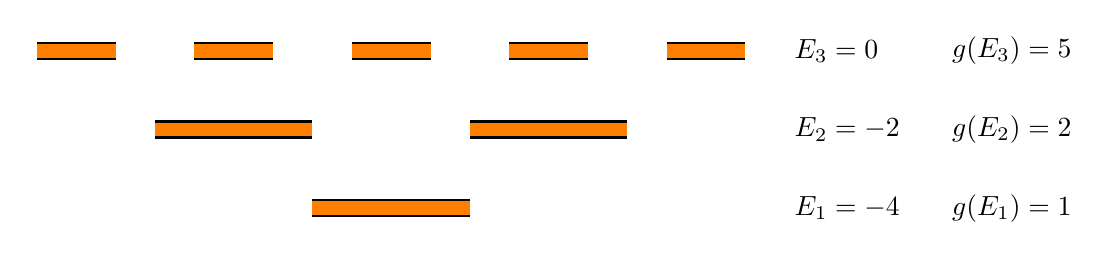
\begin{tikzpicture}
    \tikzset{level/.style   = {thick,
        double          = orange,
        double distance = 5pt}}
    
    \def\Espace{9};
    \def\Gspace{11};
    
    % Draw the energy levels.
    \draw[level] (3,0)  -- (5,0) node[right]{};
    \draw[] (\Espace,0) node[right] {$E_1=-4$};
    \draw[] (\Gspace,0) node[right] {$g(E_1)=1$};
    
    \draw[level] (1,1) -- (3,1) node[right] {};
    \draw[level] (5,1) -- (7,1) node[right] {};
    \draw[] (\Espace,1) node[right] {$E_2=-2$};
    \draw[] (\Gspace,1) node[right] {$g(E_2)=2$};
    
    \def\v{.5}; 
    \draw[level] (-1+\v,2) -- (0+\v,2) node[right] {};
    \draw[level] (1+\v,2) -- (2+\v,2) node[right] {};
    \draw[level] (3+\v,2) -- (4+\v,2) node[right] {};
    \draw[level] (5+\v,2) -- (6+\v,2) node[right] {};
    \draw[level] (7+\v,2) -- (8+\v,2) node[right] {};
    \draw[] (\Espace,2) node[right] {$E_3=0$};
    \draw[] (\Gspace,2) node[right] {$g(E_3)=5$};
  \end{tikzpicture}
}

\newcommand{\TIKZenergylevelSHORT}{

  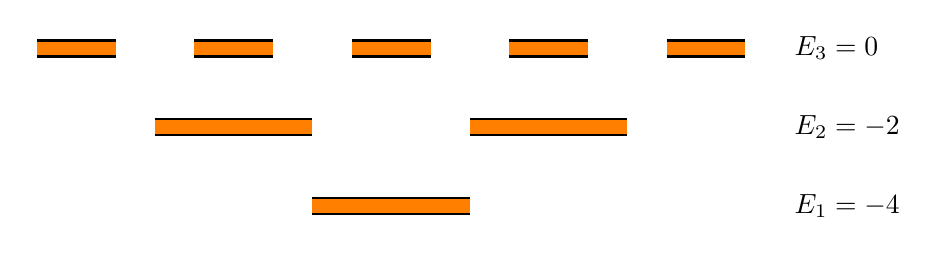
\begin{tikzpicture}
    \tikzset{level/.style   = {thick,
        double          = orange,
        double distance = 5pt,
        scale = 1.
        }}
    
    \def\Espace{9};
    \def\Gspace{11};
    
    % Draw the energy levels.
    \draw[level] (3,0)  -- (5,0) node[right]{};
    \draw[] (\Espace,0) node[right] {$E_1=-4$};
   
    \draw[level] (1,1) -- (3,1) node[right] {};
    \draw[level] (5,1) -- (7,1) node[right] {};
    \draw[] (\Espace,1) node[right] {$E_2=-2$};
    
    \def\v{.5}; 
    \draw[level] (-1+\v,2) -- (0+\v,2) node[right] {};
    \draw[level] (1+\v,2) -- (2+\v,2) node[right] {};
    \draw[level] (3+\v,2) -- (4+\v,2) node[right] {};
    \draw[level] (5+\v,2) -- (6+\v,2) node[right] {};
    \draw[level] (7+\v,2) -- (8+\v,2) node[right] {};
    \draw[] (\Espace,2) node[right] {$E_3=0$};
  \end{tikzpicture}
}


\newcommand{\TIKZgraphABC}{
  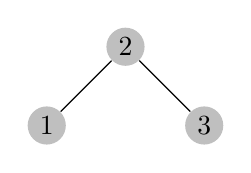
\begin{tikzpicture}[shorten >=1pt,->]
    \tikzstyle{vertex}=[circle,fill=black!25,minimum size=12pt,inner sep=2pt]
    \node[vertex] (G_1) at (-1,-1) {1};
    \node[vertex] (G_2) at (0,0)   {2};
    \node[vertex] (G_3) at (1,-1)  {3};
    \draw (G_1) -- (G_2) -- (G_3) -- cycle;
  \end{tikzpicture}
}

\newcommand{\TIKZgraphAB}{
  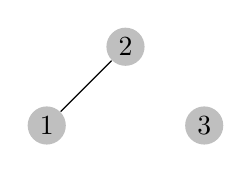
\begin{tikzpicture}[shorten >=1pt,->]
    \tikzstyle{vertex}=[circle,fill=black!25,minimum size=12pt,inner sep=2pt]
    \node[vertex] (G_1) at (-1,-1) {1};
    \node[vertex] (G_2) at (0,0)   {2};
    \node[vertex] (G_3) at (1,-1)  {3};
    \draw (G_1) -- (G_2) -- cycle;
  \end{tikzpicture}
}

\newcommand{\TIKZgraphBC}{
  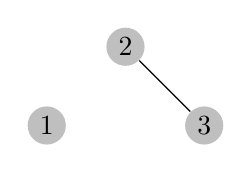
\begin{tikzpicture}[shorten >=1pt,->]
    \tikzstyle{vertex}=[circle,fill=black!25,minimum size=12pt,inner sep=2pt]
    \node[vertex] (G_1) at (-1,-1) {1};
    \node[vertex] (G_2) at (0,0)   {2};
    \node[vertex] (G_3) at (1,-1)  {3};
    \draw (G_2) -- (G_3) -- cycle;
  \end{tikzpicture}
}

\newcommand{\TIKZgraphC}{
  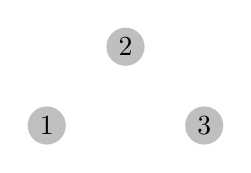
\begin{tikzpicture}[shorten >=1pt,->]
    \tikzstyle{vertex}=[circle,fill=black!25,minimum size=12pt,inner sep=2pt]
    \node[vertex] (G_1) at (-1,-1) {1};
    \node[vertex] (G_2) at (0,0)   {2};
    \node[vertex] (G_3) at (1,-1)  {3};
  \end{tikzpicture}
}


\newcommand{\TIKZgraphoneline}{
  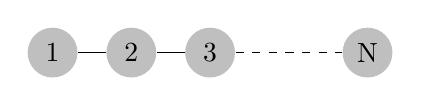
\begin{tikzpicture}[shorten >=1pt,->]
    \tikzstyle{vertex}=[circle,fill=black!25,minimum size=18pt,inner sep=2pt]
    \node[vertex] (G1) at (0,0)   {1};
    \node[vertex] (G2) at (1,0)   {2};
    \node[vertex] (G3) at (2,0)   {3};
    \node[vertex] (GN) at (4,0)   {N};
    \draw (G1) -- (G2) -- (G3) -- cycle;
    \draw[dashed] (G3) -- (GN) -- cycle;
  \end{tikzpicture}
}


\newcommand{\TIKZgraphtwoline}{
  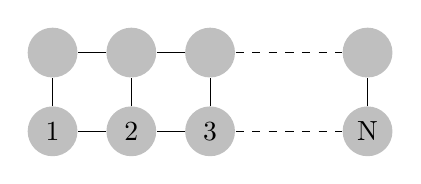
\begin{tikzpicture}[shorten >=1pt,->]
    \tikzstyle{vertex}=[circle,fill=black!25,minimum size=18pt,inner sep=2pt]
    \node[vertex] (G1) at (0,0)   {1};
    \node[vertex] (G2) at (1,0)   {2};
    \node[vertex] (G3) at (2,0)   {3};
    \node[vertex] (GN) at (4,0)   {N};
    \draw (G1) -- (G2) -- (G3) -- cycle;
    \draw[dashed] (G3) -- (GN) -- cycle;

    \node[vertex] (GN1) at (0,1)   {};
    \node[vertex] (GN2) at (1,1)   {};
    \node[vertex] (GN3) at (2,1)   {};
    \node[vertex] (G2N) at (4,1)   {};
    
    \draw (GN1) -- (GN2) -- (GN3) -- cycle;
    \draw (GN) -- (G2N) -- cycle;
    \draw (G1) -- (GN1) -- cycle;
    \draw (G2) -- (GN2) -- cycle;
    \draw (G3) -- (GN3) -- cycle;
    \draw (GN) -- (G2N) -- cycle;

    \draw[dashed] (GN3) -- (G2N) -- cycle;


  \end{tikzpicture}
}



\newcommand{\TIKZtwoladdera}{
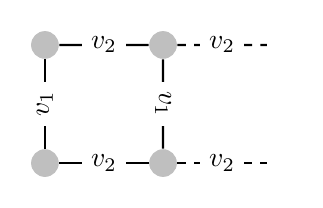
\begin{tikzpicture}[scale=\tikzpicscale]
    \node[vertex] (G1) at (0,0)   {};
    \node[vertex] (G2) at (1,0)   {};
    \node[vertex] (GA) at (0,1)   {};
    \node[vertex] (GB) at (1,1)   {};
	 \Edge[label=$v_2$](G1)(G2)
	 \Edge[label=$v_2$](GA)(GB)
	 \Edge[label=$v_1$](G1)(GA)
	 \Edge[label=$v_1$](G2)(GB)
    \node[Nvertex] (G3) at (2,0)   {};
    \node[Nvertex] (GC) at (2,1)   {};
	 \tikzstyle{EdgeStyle}=[dashed]
	 \Edge[label=$v_2$](G2)(G3)
	 \Edge[label=$v_2$](GB)(GC)
\end{tikzpicture}
}

\newcommand{\TIKZtwoladderb}{
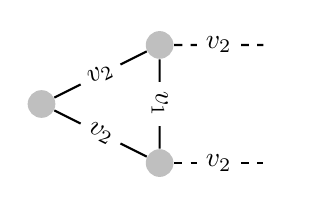
\begin{tikzpicture}[scale=\tikzpicscale]
    \node[vertex] (G2) at (1,0)   {};
    \node[vertex] (GB) at (1,1)   {};
    \node[vertex] (G1A) at (0,.5)   {};
	 \Edge[label=$v_2$](G1A)(G2)
	 \Edge[label=$v_2$](G1A)(GB)
	 \Edge[label=$v_1$](G2)(GB)
    \node[Nvertex] (G3) at (2,0)   {};
    \node[Nvertex] (GC) at (2,1)   {};
	 \tikzstyle{EdgeStyle}=[dashed]
	 \Edge[label=$v_2$](G2)(G3)
	 \Edge[label=$v_2$](GB)(GC)
\end{tikzpicture}
}

\newcommand{\TIKZtwoladderc}{
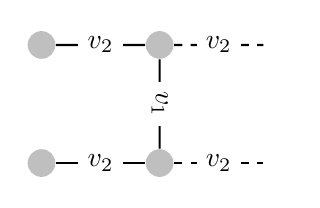
\begin{tikzpicture}[scale=\tikzpicscale]
    \node[vertex] (G1) at (0,0)   {};
    \node[vertex] (G2) at (1,0)   {};
    \node[vertex] (GA) at (0,1)   {};
    \node[vertex] (GB) at (1,1)   {};
	 \Edge[label=$v_2$](G1)(G2)
	 \Edge[label=$v_2$](GA)(GB)
	 %\Edge[label=$v_1$](G1)(GA)
	 \Edge[label=$v_1$](G2)(GB)
    \node[Nvertex] (G3) at (2,0)   {};
    \node[Nvertex] (GC) at (2,1)   {};
	 \tikzstyle{EdgeStyle}=[dashed]
	 \Edge[label=$v_2$](G2)(G3)
	 \Edge[label=$v_2$](GB)(GC)
\end{tikzpicture}
}

\newcommand{\TIKZtwoladderd}{
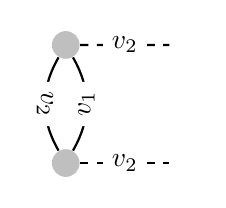
\begin{tikzpicture}[scale=\tikzpicscale]
    \node[vertex] (G2) at (1,0)   {};
    \node[vertex] (GB) at (1,1)   {};
	 %\Edge[label=$v_1$](G1)(GA)
	\tikzstyle{EdgeStyle}=[bend left]
	\Edge[label=$v_2$](G2)(GB)
  	\tikzstyle{EdgeStyle}=[bend right]
	\Edge[label=$v_1$](G2)(GB)
    \node[Nvertex] (G3) at (2,0)   {};
    \node[Nvertex] (GC) at (2,1)   {};
	 \tikzstyle{EdgeStyle}=[dashed]
	 \Edge[label=$v_2$](G2)(G3)
	 \Edge[label=$v_2$](GB)(GC)
\end{tikzpicture}
}

\newcommand{\TIKZtwoladdere}{
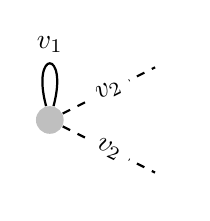
\begin{tikzpicture}[scale=\tikzpicscale]
    \node[vertex] (G2B) at (1,.5)   {};
	 %\Edge[label=$v_1$](G1)(GA)
	\tikzstyle{EdgeStyle}=[loop above]
	\Edge[label=$v_1$](G2B)(G2B)
   \node[Nvertex] (G3) at (2,0)   {};
   \node[Nvertex] (GC) at (2,1)   {};
	\tikzstyle{EdgeStyle}=[dashed]
	\Edge[label=$v_2$](G2B)(G3)
	\Edge[label=$v_2$](G2B)(GC)
\end{tikzpicture}
}

\newcommand{\TIKZtwoladderf}{
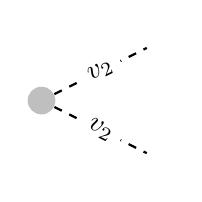
\begin{tikzpicture}[scale=\tikzpicscale]
    \node[vertex] (G2B) at (1,.5)   {};
   \node[Nvertex] (G3) at (2,0)   {};
   \node[Nvertex] (GC) at (2,1)   {};
	\tikzstyle{EdgeStyle}=[dashed]
	\Edge[label=$v_2$](G2B)(G3)
	\Edge[label=$v_2$](G2B)(GC)
\end{tikzpicture}
}

\newcommand{\TIKZthreeladderA}{
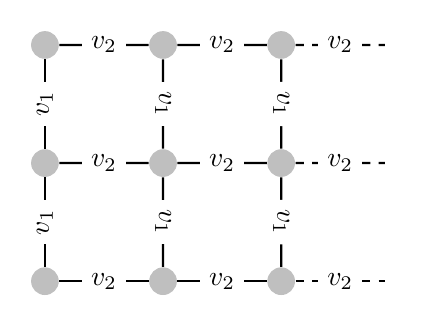
\begin{tikzpicture}[scale=\tikzpicscale]
    \node[vertex] (00) at (0,0)   {};
    \node[vertex] (10) at (1,0)   {};
	 \node[vertex] (20) at (2,0)   {};
    \node[vertex] (01) at (0,1)   {};
    \node[vertex] (11) at (1,1)   {};
    \node[vertex] (21) at (2,1)   {};
    \node[vertex] (02) at (0,2)   {};
    \node[vertex] (12) at (1,2)   {};
    \node[vertex] (22) at (2,2)   {};
	 \Edge[label=$v_2$](00)(10)
	 \Edge[label=$v_2$](10)(20)
	 \Edge[label=$v_2$](01)(11)
	 \Edge[label=$v_2$](11)(21)
	 \Edge[label=$v_2$](02)(12)
	 \Edge[label=$v_2$](12)(22)	
	 \Edge[label=$v_1$](00)(01)
	 \Edge[label=$v_1$](10)(11)
	 \Edge[label=$v_1$](20)(21)
 	 \Edge[label=$v_1$](21)(22)
 	 \Edge[label=$v_1$](11)(12)
 	 \Edge[label=$v_1$](01)(02)
    \node[Nvertex] (n30) at (3,0)   {};
    \node[Nvertex] (n31) at (3,1)   {};
    \node[Nvertex] (n32) at (3,2)   {};
	 \tikzstyle{EdgeStyle}=[dashed]
	 \Edge[label=$v_2$](20)(n30)
	 \Edge[label=$v_2$](21)(n31)
 	 \Edge[label=$v_2$](22)(n32)
\end{tikzpicture}
}

\newcommand{\TIKZthreeladderB}{
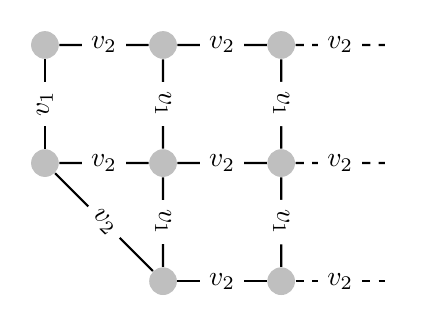
\begin{tikzpicture}[scale=\tikzpicscale]
%    \node[vertex] (00) at (0,0)   {};
    \node[vertex] (10) at (1,0)   {};
	 \node[vertex] (20) at (2,0)   {};
    \node[vertex] (01) at (0,1)   {};
    \node[vertex] (11) at (1,1)   {};
    \node[vertex] (21) at (2,1)   {};
    \node[vertex] (02) at (0,2)   {};
    \node[vertex] (12) at (1,2)   {};
    \node[vertex] (22) at (2,2)   {};
	 \Edge[label=$v_2$](01)(10)
	 \Edge[label=$v_2$](10)(20)
	 \Edge[label=$v_2$](01)(11)
	 \Edge[label=$v_2$](11)(21)
	 \Edge[label=$v_2$](02)(12)
	 \Edge[label=$v_2$](12)(22)	
%)	 \Edge[label=$v_1$](00)(01)
	 \Edge[label=$v_1$](10)(11)
	 \Edge[label=$v_1$](20)(21)
 	 \Edge[label=$v_1$](21)(22)
 	 \Edge[label=$v_1$](11)(12)
 	 \Edge[label=$v_1$](01)(02)
    \node[Nvertex] (n30) at (3,0)   {};
    \node[Nvertex] (n31) at (3,1)   {};
    \node[Nvertex] (n32) at (3,2)   {};
	 \tikzstyle{EdgeStyle}=[dashed]
	 \Edge[label=$v_2$](20)(n30)
	 \Edge[label=$v_2$](21)(n31)
 	 \Edge[label=$v_2$](22)(n32)
\end{tikzpicture}
}

\newcommand{\TIKZthreeladderC}{
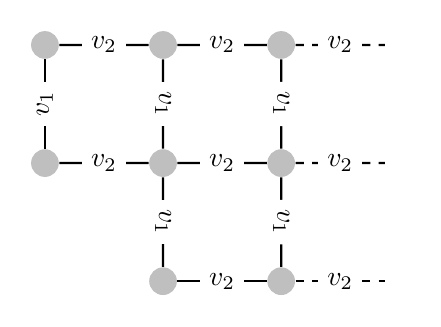
\begin{tikzpicture}[scale=\tikzpicscale]
%    \node[vertex] (00) at (0,0)   {};
    \node[vertex] (10) at (1,0)   {};
	 \node[vertex] (20) at (2,0)   {};
    \node[vertex] (01) at (0,1)   {};
    \node[vertex] (11) at (1,1)   {};
    \node[vertex] (21) at (2,1)   {};
    \node[vertex] (02) at (0,2)   {};
    \node[vertex] (12) at (1,2)   {};
    \node[vertex] (22) at (2,2)   {};
%	 \Edge[label=$v_2$](01)(10)
	 \Edge[label=$v_2$](10)(20)
	 \Edge[label=$v_2$](01)(11)
	 \Edge[label=$v_2$](11)(21)
	 \Edge[label=$v_2$](02)(12)
	 \Edge[label=$v_2$](12)(22)	
%)	 \Edge[label=$v_1$](00)(01)
	 \Edge[label=$v_1$](10)(11)
	 \Edge[label=$v_1$](20)(21)
 	 \Edge[label=$v_1$](21)(22)
 	 \Edge[label=$v_1$](11)(12)
 	 \Edge[label=$v_1$](01)(02)
    \node[Nvertex] (n30) at (3,0)   {};
    \node[Nvertex] (n31) at (3,1)   {};
    \node[Nvertex] (n32) at (3,2)   {};
	 \tikzstyle{EdgeStyle}=[dashed]
	 \Edge[label=$v_2$](20)(n30)
	 \Edge[label=$v_2$](21)(n31)
 	 \Edge[label=$v_2$](22)(n32)
\end{tikzpicture}
}

\newcommand{\TIKZthreeladderD}{
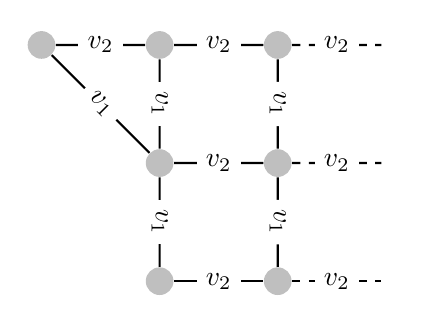
\begin{tikzpicture}[scale=\tikzpicscale]
%    \node[vertex] (00) at (0,0)   {};
    \node[vertex] (10) at (1,0)   {};
	 \node[vertex] (20) at (2,0)   {};
%    \node[vertex] (01) at (0,1)   {};
    \node[vertex] (11) at (1,1)   {};
    \node[vertex] (21) at (2,1)   {};
    \node[vertex] (02) at (0,2)   {};
    \node[vertex] (12) at (1,2)   {};
    \node[vertex] (22) at (2,2)   {};
%	 \Edge[label=$v_2$](01)(10)
	 \Edge[label=$v_2$](10)(20)
%	 \Edge[label=$v_2$](01)(11)
	 \Edge[label=$v_2$](11)(21)
	 \Edge[label=$v_2$](02)(12)
	 \Edge[label=$v_2$](12)(22)	
%)	 \Edge[label=$v_1$](00)(01)
	 \Edge[label=$v_1$](10)(11)
	 \Edge[label=$v_1$](20)(21)
 	 \Edge[label=$v_1$](21)(22)
 	 \Edge[label=$v_1$](11)(12)
 	 \Edge[label=$v_1$](11)(02)
    \node[Nvertex] (n30) at (3,0)   {};
    \node[Nvertex] (n31) at (3,1)   {};
    \node[Nvertex] (n32) at (3,2)   {};
	 \tikzstyle{EdgeStyle}=[dashed]
	 \Edge[label=$v_2$](20)(n30)
	 \Edge[label=$v_2$](21)(n31)
 	 \Edge[label=$v_2$](22)(n32)
\end{tikzpicture}
}

\newcommand{\TIKZthreeladderE}{
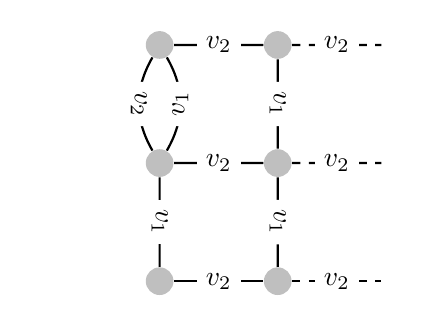
\begin{tikzpicture}[scale=\tikzpicscale]
    \node[Nvertex] (00) at (0,0)   {};
    \node[vertex] (10) at (1,0)   {};
	 \node[vertex] (20) at (2,0)   {};
%    \node[vertex] (01) at (0,1)   {};
    \node[vertex] (11) at (1,1)   {};
    \node[vertex] (21) at (2,1)   {};
%    \node[vertex] (02) at (0,2)   {};
    \node[vertex] (12) at (1,2)   {};
    \node[vertex] (22) at (2,2)   {};
%	 \Edge[label=$v_2$](01)(10)
	 \Edge[label=$v_2$](10)(20)
%	 \Edge[label=$v_2$](01)(11)
	 \Edge[label=$v_2$](11)(21)
%	 \Edge[label=$v_2$](02)(12)
	 \Edge[label=$v_2$](12)(22)	
%)	 \Edge[label=$v_1$](00)(01)
	 \Edge[label=$v_1$](10)(11)
	 \Edge[label=$v_1$](20)(21)
 	 \Edge[label=$v_1$](21)(22)
% 	 \Edge[label=$v_1$](11)(02)
    \node[Nvertex] (n30) at (3,0)   {};
    \node[Nvertex] (n31) at (3,1)   {};
    \node[Nvertex] (n32) at (3,2)   {};
	 \tikzstyle{EdgeStyle}=[dashed]
	 \Edge[label=$v_2$](20)(n30)
	 \Edge[label=$v_2$](21)(n31)
 	 \Edge[label=$v_2$](22)(n32)
 	 \tikzstyle{EdgeStyle}=[bend left]
  	 \Edge[label=$v_2$](11)(12)
  	 \tikzstyle{EdgeStyle}=[bend right]
  	 \Edge[label=$v_1$](11)(12)
\end{tikzpicture}
}

\newcommand{\TIKZthreeladderF}{
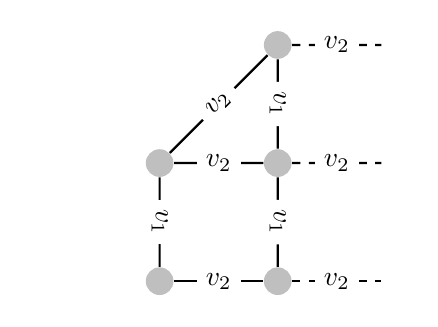
\begin{tikzpicture}[scale=\tikzpicscale]
    \node[Nvertex] (00) at (0,0)   {};
    \node[vertex] (10) at (1,0)   {};
	 \node[vertex] (20) at (2,0)   {};
%    \node[vertex] (01) at (0,1)   {};
    \node[vertex] (11) at (1,1)   {};
    \node[vertex] (21) at (2,1)   {};
%    \node[vertex] (02) at (0,2)   {};
%    \node[vertex] (12) at (1,2)   {};
    \node[vertex] (22) at (2,2)   {};
%	 \Edge[label=$v_2$](01)(10)
	 \Edge[label=$v_2$](10)(20)
%	 \Edge[label=$v_2$](01)(11)
	 \Edge[label=$v_2$](11)(21)
%	 \Edge[label=$v_2$](02)(12)
	 \Edge[label=$v_2$](11)(22)	
%)	 \Edge[label=$v_1$](00)(01)
	 \Edge[label=$v_1$](10)(11)
	 \Edge[label=$v_1$](20)(21)
 	 \Edge[label=$v_1$](21)(22)
% 	 \Edge[label=$v_1$](11)(02)
    \node[Nvertex] (n30) at (3,0)   {};
    \node[Nvertex] (n31) at (3,1)   {};
    \node[Nvertex] (n32) at (3,2)   {};
	 \tikzstyle{EdgeStyle}=[dashed]
	 \Edge[label=$v_2$](20)(n30)
	 \Edge[label=$v_2$](21)(n31)
 	 \Edge[label=$v_2$](22)(n32)
  	 %\tikzstyle{EdgeStyle}=[loop above]
  	 %\Edge[label=$v_1$](11)(11)
\end{tikzpicture}
}

\newcommand{\TIKZthreeladderG}{
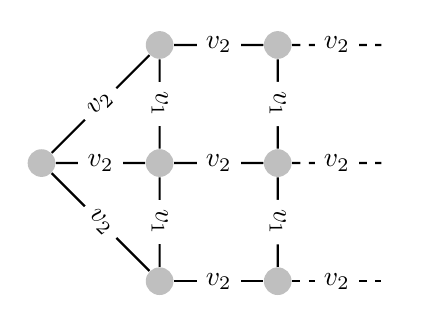
\begin{tikzpicture}[scale=\tikzpicscale]
%    \node[vertex] (00) at (0,0)   {};
    \node[vertex] (10) at (1,0)   {};
	 \node[vertex] (20) at (2,0)   {};
    \node[vertex] (01) at (0,1)   {};
    \node[vertex] (11) at (1,1)   {};
    \node[vertex] (21) at (2,1)   {};
%    \node[vertex] (02) at (0,2)   {};
    \node[vertex] (12) at (1,2)   {};
    \node[vertex] (22) at (2,2)   {};
	 \Edge[label=$v_2$](01)(10)
	 \Edge[label=$v_2$](10)(20)
	 \Edge[label=$v_2$](01)(11)
	 \Edge[label=$v_2$](11)(21)
	 \Edge[label=$v_2$](01)(12)
	 \Edge[label=$v_2$](12)(22)	
%)	 \Edge[label=$v_1$](00)(01)
	 \Edge[label=$v_1$](10)(11)
	 \Edge[label=$v_1$](20)(21)
 	 \Edge[label=$v_1$](21)(22)
 	 \Edge[label=$v_1$](11)(12)
% 	 \Edge[label=$v_1$](01)(02)
    \node[Nvertex] (n30) at (3,0)   {};
    \node[Nvertex] (n31) at (3,1)   {};
    \node[Nvertex] (n32) at (3,2)   {};
	 \tikzstyle{EdgeStyle}=[dashed]
	 \Edge[label=$v_2$](20)(n30)
	 \Edge[label=$v_2$](21)(n31)
 	 \Edge[label=$v_2$](22)(n32)
\end{tikzpicture}
}

\newcommand{\TIKZthreeladderH}{
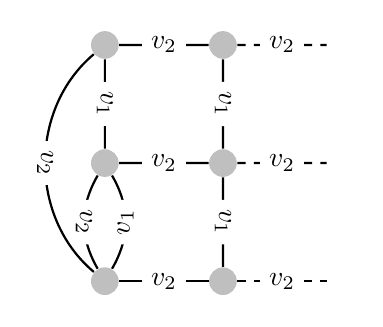
\begin{tikzpicture}[scale=\tikzpicscale]
%    \node[vertex] (00) at (0,0)   {};
    \node[vertex] (10) at (1,0)   {};
	 \node[vertex] (20) at (2,0)   {};
%    \node[vertex] (01) at (0,1)   {};
    \node[vertex] (11) at (1,1)   {};
    \node[vertex] (21) at (2,1)   {};
%    \node[vertex] (02) at (0,2)   {};
    \node[vertex] (12) at (1,2)   {};
    \node[vertex] (22) at (2,2)   {};
	 \Edge[label=$v_2$](10)(20)
%	 \Edge[label=$v_2$](01)(11)
	 \Edge[label=$v_2$](11)(21)
%	 \Edge[label=$v_2$](01)(12)
	 \Edge[label=$v_2$](12)(22)	
%)	 \Edge[label=$v_1$](00)(01)
	 \Edge[label=$v_1$](20)(21)
 	 \Edge[label=$v_1$](21)(22)
 	 \Edge[label=$v_1$](11)(12)
% 	 \Edge[label=$v_1$](01)(02)
    \node[Nvertex] (n30) at (3,0)   {};
    \node[Nvertex] (n31) at (3,1)   {};
    \node[Nvertex] (n32) at (3,2)   {};
	 \tikzstyle{EdgeStyle}=[dashed]
	 \Edge[label=$v_2$](20)(n30)
	 \Edge[label=$v_2$](21)(n31)
 	 \Edge[label=$v_2$](22)(n32)
 	 
 	 \tikzstyle{EdgeStyle}=[bend left]
 	 \Edge[label=$v_2$](10)(11)
  	 \tikzstyle{EdgeStyle}=[bend left=50]
 	 \Edge[label=$v_2$](10)(12)
  	 %\Edge[label=$v_2$](11)(12)
 	 \tikzstyle{EdgeStyle}=[bend right]
	 \Edge[label=$v_1$](10)(11)
\end{tikzpicture}
}

\newcommand{\TIKZthreeladderI}{
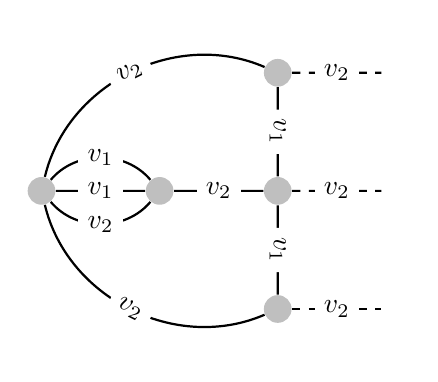
\begin{tikzpicture}[scale=\tikzpicscale]
%    \node[vertex] (00) at (0,0)   {};
%    \node[vertex] (10) at (1,0)   {};
	 \node[vertex] (20) at (2,0)   {};
    \node[vertex] (01) at (0,1)   {};
    \node[vertex] (11) at (1,1)   {};
    \node[vertex] (21) at (2,1)   {};
%    \node[vertex] (02) at (0,2)   {};
%    \node[vertex] (12) at (1,2)   {};
    \node[vertex] (22) at (2,2)   {};
%	 \Edge[label=$v_2$](01)(10)
%	 \Edge[label=$v_2$](10)(20)
%	 \Edge[label=$v_2$](01)(21)
	 \Edge[label=$v_2$](11)(21)
%	 \Edge[label=$v_2$](12)(22)	
%)	 \Edge[label=$v_1$](00)(01)
%	 \Edge[label=$v_1$](10)(11)
	 \Edge[label=$v_1$](20)(21)
 	 \Edge[label=$v_1$](21)(22)
% 	 \Edge[label=$v_1$](11)(12)
% 	 \Edge[label=$v_1$](01)(02)
    \node[Nvertex] (n30) at (3,0)   {};
    \node[Nvertex] (n31) at (3,1)   {};
    \node[Nvertex] (n32) at (3,2)   {};
	 \tikzstyle{EdgeStyle}=[dashed]
	 \Edge[label=$v_2$](20)(n30)
	 \Edge[label=$v_2$](21)(n31)
 	 \Edge[label=$v_2$](22)(n32)

	 \tikzstyle{EdgeStyle}=[]
	 \Edge[label=$v_1$](01)(11)
  	 \tikzstyle{EdgeStyle}=[bend left=50]
	 \Edge[label=$v_2$](01)(22)
 	 \Edge[label=$v_1$](01)(11)
  	 \tikzstyle{EdgeStyle}=[bend right=50]
 	 \Edge[label=$v_2$](01)(20)
 	 \Edge[label=$v_2$](01)(11)
\end{tikzpicture}
}


\newcommand{\TIKZthreeladderJ}{
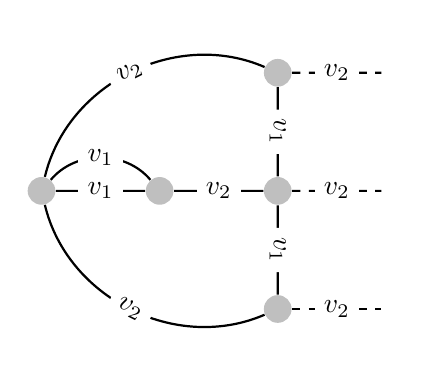
\begin{tikzpicture}[scale=\tikzpicscale]
%    \node[vertex] (00) at (0,0)   {};
%    \node[vertex] (10) at (1,0)   {};
	 \node[vertex] (20) at (2,0)   {};
    \node[vertex] (01) at (0,1)   {};
    \node[vertex] (11) at (1,1)   {};
    \node[vertex] (21) at (2,1)   {};
%    \node[vertex] (02) at (0,2)   {};
%    \node[vertex] (12) at (1,2)   {};
    \node[vertex] (22) at (2,2)   {};
%	 \Edge[label=$v_2$](01)(10)
%	 \Edge[label=$v_2$](10)(20)
%	 \Edge[label=$v_2$](01)(21)
	 \Edge[label=$v_2$](11)(21)
%	 \Edge[label=$v_2$](12)(22)	
%)	 \Edge[label=$v_1$](00)(01)
%	 \Edge[label=$v_1$](10)(11)
	 \Edge[label=$v_1$](20)(21)
 	 \Edge[label=$v_1$](21)(22)
% 	 \Edge[label=$v_1$](11)(12)
% 	 \Edge[label=$v_1$](01)(02)
    \node[Nvertex] (n30) at (3,0)   {};
    \node[Nvertex] (n31) at (3,1)   {};
    \node[Nvertex] (n32) at (3,2)   {};
	 \tikzstyle{EdgeStyle}=[dashed]
	 \Edge[label=$v_2$](20)(n30)
	 \Edge[label=$v_2$](21)(n31)
 	 \Edge[label=$v_2$](22)(n32)

	 \tikzstyle{EdgeStyle}=[]
	 \Edge[label=$v_1$](01)(11)
  	 \tikzstyle{EdgeStyle}=[bend left=50]
	 \Edge[label=$v_2$](01)(22)
 	 \Edge[label=$v_1$](01)(11)
  	 \tikzstyle{EdgeStyle}=[bend right=50]
 	 \Edge[label=$v_2$](01)(20)
% 	 \Edge[label=$v_2$](01)(11)
\end{tikzpicture}
}

\newcommand{\TIKZoneladderA}{
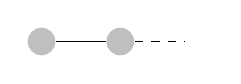
\begin{tikzpicture}[shorten >=1pt,->]
    \tikzstyle{vertex}=[circle,fill=black!25,minimum size=10pt,inner sep=2pt]
    \tikzstyle{nullvertex}=[circle,fill=white!25,minimum size=10pt,inner sep=2pt]
    \node[vertex] (G1) at (0,0)   {};
    \node[vertex] (G2) at (1,0)   {};
    \node[nullvertex] (GX) at (2,0)   {};
    \draw (G1) -- (G2) -- cycle;
    \draw[dashed] (G2) -- (GX) -- cycle;
\end{tikzpicture}
}

\newcommand{\TIKZoneladderB}{
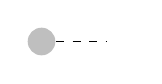
\begin{tikzpicture}[shorten >=1pt,->]
    \tikzstyle{vertex}=[circle,fill=black!25,minimum size=10pt,inner sep=2pt]
    \tikzstyle{nullvertex}=[circle,fill=white!25,minimum size=10pt,inner sep=2pt]
    \node[vertex] (G2) at (1,0)   {};
    \node[nullvertex] (GX) at (2,0)   {};
    \draw[dashed] (G2) -- (GX) -- cycle;
\end{tikzpicture}
}

\newcommand{\TIKZoneladderC}{

\begin{tikzpicture}[shorten >=1pt,->]
    \tikzstyle{vertex}=[circle,fill=black!25,minimum size=10pt,inner sep=2pt]
    \tikzstyle{nullvertex}=[circle,fill=white!25,minimum size=10pt,inner sep=2pt]
    \node[vertex] (G1) at (0,0)   {};
    \node[vertex] (G2) at (1,0)   {};
    \node[nullvertex] (GX) at (2,0)   {};
    %\draw (G1) -- (G2) -- cycle;
    \draw[dashed] (G2) -- (GX) -- cycle;
\end{tikzpicture}
}

\newcommand{\TIKZpetersengraph} {
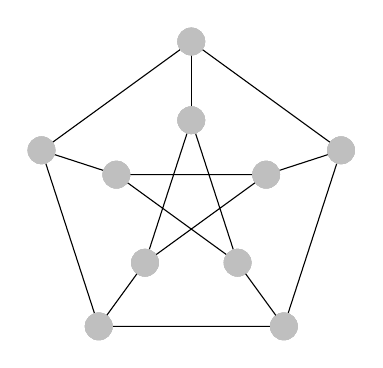
\begin{tikzpicture}[]
    \tikzstyle{vertex}=[circle,fill=black!25,minimum size=10pt,inner sep=2pt]
            
\draw (18:2cm) -- (90:2cm) -- (162:2cm) -- (234:2cm) -- (306:2cm) -- cycle;
\draw (18:1cm) -- (162:1cm) -- (306:1cm) -- (90:1cm) -- (234:1cm) -- cycle;
\foreach \x in {18,90,162,234,306}{
\draw (\x:1cm) -- (\x:2cm);

    \node[vertex] at (18:2cm) {};
    \node[vertex] at (90:2cm) {};
    \node[vertex] at (162:2cm) {};
    \node[vertex] at (234:2cm) {};
    \node[vertex] at (306:2cm) {};
    \node[vertex] at (18:1cm) {};
    \node[vertex] at (162:1cm) {};
    \node[vertex] at (306:1cm) {};
    \node[vertex] at (90:1cm) {};
    \node[vertex] at (234:1cm) {};

%\draw (\x:2cm) circle (2pt);
%\draw (\x:1cm) circle (2pt);
}
\end{tikzpicture}
}

\newcommand{\TIKZFLWmacrostates} {

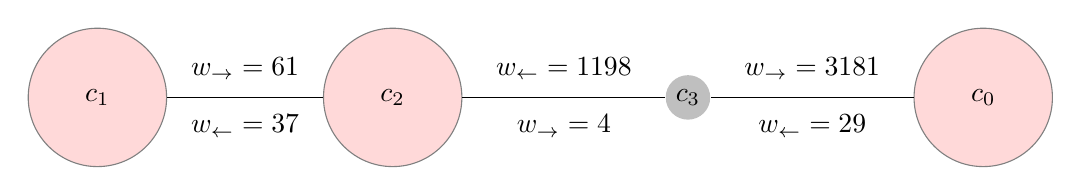
\begin{tikzpicture}[scale=\tikzpicscale]

  \node[big_vertex] (c1) at (0,0)   {$c_1$};
  \node[big_vertex] (c2) at (1*\vertexshiftamount,0)   {$c_2$};
  \node[vertex]    (c3) at (2*\vertexshiftamount,0)   {$c_3$};
  \node[big_vertex] (c0) at (3*\vertexshiftamount,0)   {$c_0$};
  
  \draw [] (c0) -> node[above=.1cm] {$w_{\rightarrow}=3181$} (c3);
  \draw [] (c0) -> node[below=.1cm] {$w_{\leftarrow}=29$} (c3);

  \draw [] (c2) -> node[above=.1cm] {$w_{\leftarrow}=1198$} (c3);  
  \draw [] (c2) -> node[below=.1cm] {$w_{\rightarrow}=4$} (c3);
  
  \draw [] (c2) -- node[below=.1cm] {$w_{\leftarrow}=37$} (c1);
  \draw [] (c2) -- node[above=.1cm] {$w_{\rightarrow}=61$} (c1);
\end{tikzpicture}
}

\newcommand{\TIKZbetahairpinNativestate} {
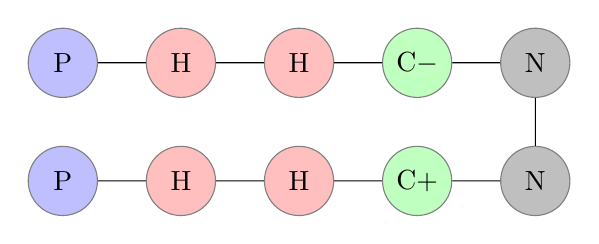
\begin{tikzpicture}[scale=\tikzpicscale]
    \tikzstyle{hvertex}=[circle,fill=red!25,minimum size=25pt,inner sep=2pt,draw=black!50]
    \tikzstyle{pvertex}=[circle,fill=blue!25,minimum size=25pt,inner sep=2pt,draw=black!50]
    \tikzstyle{cpvertex}=[circle,fill=green!25,minimum size=25pt,inner sep=2pt,draw=black!50]
    \tikzstyle{nvertex}=[circle,fill=black!25,minimum size=25pt,inner sep=2pt,draw=black!50]

    \node[pvertex] (r0) at (0,0)   {\chem{P}};
    \node[hvertex] (r1) at (1,0)   {\chem{H}};
    \node[hvertex] (r2) at (2,0)   {\chem{H}};
    \node[cpvertex] (r3) at (3,0)   {\chem{C+}};
    \node[nvertex] (r4) at (4,0)   {\chem{N}};
    \node[nvertex] (r5) at (4,1)   {\chem{N}};
    \node[cpvertex] (r6) at (3,1)   {\chem{C-}};
    \node[hvertex] (r7) at (2,1)   {\chem{H}};
    \node[hvertex] (r8) at (1,1)   {\chem{H}};
    \node[pvertex] (r9) at (0,1)   {\chem{P}};

    \draw [] (r0)--(r1)--(r2)--(r3)--(r4)--(r5)--(r6)--(r7)--(r8)--(r9)--cycle;
   
\end{tikzpicture}
}


\newcommand{\TIKZbetahairpinMacrostates} {
\begin{tikzpicture}[scale=\tikzpicscale]
    \node[macrostate_vertex] (R) at (0,0)   {
    \begin{minipage}{3.1cm}
    \includegraphics[width=1.5 cm]{supplement/beta_cluster_example_2/pictures/21/state_cluster_shapes_150.pdf} 
    \includegraphics[width=1.5 cm]{supplement/beta_cluster_example_2/pictures/21/state_cluster_shapes_17.pdf} \\
    \includegraphics[width=1.5 cm]{supplement/beta_cluster_example_2/pictures/21/state_cluster_shapes_32.pdf} 
    \includegraphics[width=1.5 cm]{supplement/beta_cluster_example_2/pictures/21/state_cluster_shapes_200.pdf} \\
  	 $c_\chem{R}$ random coil
    \end{minipage}
    };
    \node[macrostate_vertex] (I) at (1.5*\vertexshiftamount,0)   {
    \begin{minipage}{3.1cm} \centering
    \includegraphics[width=2 cm]{supplement/beta_cluster_example_2/pictures/saved_macrostates/intermed.png} \\
  	 $c_\chem{I}$ intermediate \\ (turn formation)
    \end{minipage}
	 };
    \node[macrostate_vertex] (F) at (3*\vertexshiftamount,0)   
    {
    \begin{minipage}{3.1cm} \centering
    \includegraphics[width=2.5 cm]{supplement/beta_cluster_example_2/pictures/saved_macrostates/native.png} \\
  	 $c_\chem{F}$ native state
    \end{minipage}
    };

  \tikzstyle{EdgeStyle}=[bend right]
  \Edge[label=$\B{S}_{\chem{R I}}$](R)(I)
  \Edge[label=$\B{S}_{\chem{I R}}$](I)(R)
  
  \tikzstyle{EdgeStyle}=[]
  \Edge[label=$\B{S}_{\chem{I F}}$](I)(F)
  
\end{tikzpicture}
}


%\end{comment}


\begin{document}

\begin{preamble}

\iffinal{}{\newpage}
\begin{DUTdedications}
%
\vspace*{\fill}
%
\begin{center}
\setstretch{2}
\begin{minipage}{8 cm}
\begin{center}
\hrulefill\\
This thesis is dedicated to Cara Hoppe.\\ 
I respect her as my peer,\\
and cherish her as my wife.\\
Her love and support made this work possible. \\
%\hrulefill\hspace{0.2cm} \leafNE \hspace{0.2cm} \hrulefill
\hrulefill
\vspace{6em}
\end{center}
\end{minipage}
\end{center} 
%
\vspace*{\fill}
%
\end{DUTdedications} 
\iffinal{}{\newpage}

\begin{acknowledgments}
  \iffinal{}{\setstretch{1.5}}
The completion of this thesis could not have been done without the tireless support of my advisor, Dr. Jian-Min Yuan. I am deeply indebted for the support he has provided over the years. As a mentor, he helped me develop my skills as a scientist and honed my critical thinking. He is an endless source of new ideas and has taught me how to effectively communicate in the scientific world. 

I would also like to thank the physics department at Drexel for helping me prepare for the journey ahead. In particular, both Dr. Michel Vallieres and Dr. Robert Gilmore have been gracious enough to spend many afternoons discussing every interesting theory I've come across. Their insights and enthusiasm for physics and mathematics is inspiring. 

I would like to thank my family, my wife, Cara Hoppe, and my children, Hazel and Jackson Hoppe. They cheerfully remind me of the world outside and always bring a smile to my face. Finally, I would like to thank my uncle, Fred Stein, who introduced me to physics and all its wonders at an early age.
 
  \end{acknowledgments}
  \iffinal{}{\newpage}

  \listoffigures 
  \iffinal{}{\newpage}

  \tableofcontents 
  \iffinal{}{\newpage}

  \begin{abstract}
  \iffinal{}{\setstretch{1.5}}
  \setstretch{1.5}
A protein's ultimate function and activity is determined by the unique three-dimensional structure taken by the folding process. Protein malfunction due to misfolding is the culprit of many clinical disorders, such as abnormal protein aggregations. This leads to neurodegenerative disorders like Huntington's and Alzheimer's disease. We focus on a subset of the folding problem, exploring the role and effects of entropy on the process of protein folding. Four major concepts and models are developed and each pertains to a specific aspect of the folding process: entropic forces, conformational states under crowding, aggregation, and macrostate kinetics from microstate trajectories. 

The exclusive focus on entropy is well-suited for crowding studies, as many interactions are non-specific. We show how a stabilizing entropic force can arise purely from the motion of crowders in solution. In addition we are able to make a a quantitative prediction of the crowding effect with an implicit crowding approximation using an aspherical scaled-particle theory.

In order to investigate the effects of aggregation, we derive a new operator expansion method to solve the Ising/Potts model with external fields over an arbitrary graph. Here the external fields are representative of the entropic forces. We show that this method reduces the problem of calculating the partition function to the solution of recursion relations. 

Many of the methods employed are coarse-grained approximations. As such, it is useful to have a viable method for extracting macrostate information from time series data. We develop a method to cluster the microstates into physically meaningful macrostates by grouping similar relaxation times from a transition matrix.  

Overall, the studied topics allow us to understand deeper the complicated process involving proteins.
  \end{abstract} 

	\iffinal{}{\newpage}

\end{preamble}


\begin{thesis}
  \pdfbookmark[-1]{Main Matter}{Main Matter}
  \ifdaring{\setstretch{1.3}}{}
  %\ifdaring{\setstretch{1.3}}{\setstretch{1.3}}
  
  %CHAPTER: Introduction
  \chapter{Introduction}

The practice of staining glass for decorative purposes dates to ancient Rome,
but the investigation of light matter interaction starts even back to the
begining of history for human beings, when ancient men wondered about the
source of light ,sun, or the first time to use a torch for hunting. People
never stop studying how the light interacts with our world, meanwhile, this
leads to improving our understanding and building a better world with photonic
technology. The stained-glass windows such as the one inside of the St.
Patrick's Cathedral in Fig.~\ref{StainGlass} served as a 'poor man's Bible' in
the Middle Ages, allowing believers who could not read Latin to learn the story
of the Gospels.  The term stained glass refers to glass that has been coloured
by adding metallic salts during its manufacture. Then this coloured glass is
crafted into stained glass windows in which small pieces of glass are arranged
to form patterns or pictures. Even nowadays, people are still surprised about
how beautiful they are and wondering how the light interact with these pieces
of art crafts. Besides the arts, lighting technology is also evolving very
rapidly, from the ancient torchs to the bulb that Thomas Edison invented and to
the modern LEDs such as the ones also shown in Fig.~\ref{StainGlass}. From
blackbody radiation to electroluminescence, i.e., from thermal radiation to
radiative recombination, we are now capable of generating light more
efficiently.

\begin{figure}
  \caption{The Stained-glass window and the top modern lamps inside of the St. Patrick's Cathedral, 5th Ave, New York, NY.}
  \centering
  \includegraphics[width=0.5\textwidth,height=0.5\textheight]{pictures/Introduction/StainGlass}
  \label{StainGlass}
\end{figure}

Now we find ourselves living through a new revolution in the age of information
technology, one with consequences every bit as dramatic and likely even more
profound as the data transmission by light. Electrons have served us very well
for the past few decades, but the explosion of data. The storage and the
transmission of data consumes large amount of power and time, simultaneously.
Meeting the energy needs of the communication of information, together with
storage and computation form a "grand challenge" of the information age.

One good example of huge amount of power consumption by data transmission and
computation is the data centers, which currently consume 1.5\% of global energy
production, and up to approximately 4\% of U.S. energy produced. Though the
statistics seems small, a 1000 times increase in the volume of data is
predicted by 2025~\cite{Hilbert:2011tg}. Google data center alone consumes
enough electricity to power 200,000 homes, since an average Google search or a
YouTube video or a message through Gmail uses 0.3 watt-hours of
electricity~\cite{glanz2011google}. Having efficient data computation and
transmission tools will greatly reduce the total data center power consumption
into a greener number. And the data pipelines of light can certainly be very
helpful in this regime.

\section{Background} \label{sec:intro_BG}

\subsection{Photonics and Optoelectronics}

Photonics involves the generation, control and detection of lightwaves and
photons, which are particles of light, in free space or solid.
Optoelectronics is the study and application of effects related to the
interaction of light and electronic signals, and may be considered a sub-field
of photonics. Both photonics and optoelectronics study the light, and explore a
wider variety of wavelengths besides visible lightwave range, from gamma rays
to radio, including X-rays, ultraviolet and infrared light.

The invention and development of solar
cells~\cite{sun2005organic,perlin1999space},
photodetector~\cite{razeghi1996semiconductor,rogalski2002infrared},
modulators~\cite{chen2011broadband,schuller2010plasmonics},
LEDs~\cite{spanggaard2004brief,schubert2005solid,schubert2005light} and
lasers~\cite{chow2012semiconductor,yablonovitch1987inhibited} certainly set the
example of breakthroughs due to the manipulation of photons in thin films and
semiconductor bulk crystals. The continuing success of photonic technologies
relies on the discovery of new optical materials and the miniaturization of
optoelectronic devices that feature better performance, low cost and low power
consumption. For the last few decades, countless efforts in nano-scale
materials and devices research have created a rich collection of nanostructures
where size, shape and composition can be readily controled. Many such
nanostructures exhibit fascinating optical properties that could have
significant impact in the future for photonic technology.

\subsection{Core-Shell Nanowires} \label{sec:intro_CSNW}

The primary principle for constantly miniaturizing the device is not only about
the size, but also to have better electronic and optical properties. As the
critical dimension of semiconductor solid-state devices keep shrinking, the
effect of charge carriers quantization becomes more prominent, and to be more
specific, this means the confinement of electrons or holes by constructing
quantum confined structures. At the very dawn of electronics, the idea of using
heterostructures (i.e., the structure with two layers or regions of dissimilar
crystalline semiconductors) has emerged. After Shockley proposed the idea,
Alferov and Kroemer introduced the concept that heterojuctions could possess
high injection efficiencies in comparison with homojunctions, and which we know
now is due to the confinement of carriers~\cite{alferov2000double}. It would be
very difficult today to imagine solid-state physics without semiconductor
heterostructures for both electronic-based and optical-based applications. The
heterostructures and, especially, double heterostructures, including quantum
wells, nanowires, and quantum dots, are the fundamental building blocks for
current nanoscience research as depicted in Fig.~\ref{Nanomaterials}.

\begin{figure}
  \caption{Diagram of classification of nano-materials and nano-scale structures}
  \centering
  \includegraphics[width=\textwidth]{pictures/Introduction/Nanomaterials}
  \label{Nanomaterials}
\end{figure}

Quantum well is a potential well which confines particles to only move freely
in two dimensions in stead of three dimensions, by forcing them to occupy a
planar region. These wells are typically formed in semiconductors by having a
narrower bandgap material sandwiched between two layers with wider bandgap
materials. Electrons in quantum wells are confined in two dimensions either
naturally or by doping the barrier of a quantum well, thus a two-dimensional
electron gas (2DEG) may be formed at the heterointerface. This not only
increases the density of electrons, but also causes a better performance in
optoelectronic devices such as laser diodes~\cite{nakamura1996ingan}, High
Electron Mobility Transistors (HEMTs)~\cite{kuzmik2002inaln,rosenberg19850},
photodetectors~\cite{levine1993quantum,liu2004terahertz}, and solar
cells~\cite{barnham2002quantum,ekins1999strain}.

Quantum dots, as another most common nanostructure in semiconductor physics,
exhibit much more enhanced optical properties. They are normally only several
nano-meters in size, and either synthesized or self-assembled into a bulk
solid. As the particles in the quantum dots are confined in three dimensions,
which leave them zero degree of freedom. As a result, the density of states
changes to a delta function as opposed to a smooth square root dependence that
is found in bulk materials. The narrower peak spectra and larger magnitude of
intensity make them even better candidates in the application of solar
cells~\cite{nozik2002quantum},
lasers~\cite{klimov2000optical,ustinov2003quantum} and light emitting diodes
(LEDs)~\cite{park2001band,sun2007bright}.

However, since the introduction in the 1990's, another important class of
semiconductor nanostructures has emerged: structures with cross-sections of
tens or hundreds of nano-meters and lengths up to several micro-meters. These
structures are named as 'nanowires'~\cite{xia2003one} different from quantum
dots as they are confined only in two dimensions, thus allowing electrons,
holes or photons to propagate freely along the third dimension. Besides their
own outstanding electro-optical properties, the high-aspect-ratio of these new
semiconductor nanostructures allows for the bridging of the nanoscopic and
macroscopic world. As P. Yang writes in their review paper:~\cite{Yan:2009hm}
"This nano-macro interface is fundamental to the integration of nanoscale
building blocks in electrical or optoelectronic device applications.
Conventional photonic platforms often consist of features with large
aspect-ratios such as interconnects and waveguides, typically with micrometre
dimensions. Thus, when semiconductor nanowires emerged they were immediately
recognized as one of the essential building blocks for nanophotonics."

The development of sophisticated nanowires growth
techniques~\cite{hobbs2012semiconductor,wu2001direct}, either
bottom-up~\cite{lu2007nanoelectronics,Huang:2001kv} or
top-down~\cite{park2009top}, has stimulated a large body of new work in
semiconductor nanowires over the last twenty years or so. Previously, the
research activities focused on the growth of higher quality
nanowires~\cite{Yang:2002ts} and the variation of its constituent materials. At
that time, most of the nanowires were core-only with ZnO~\cite{Yang:2002ts},
GaAs~\cite{persson2004solid}, Si~\cite{hochbaum2005controlled}, or
Ge~\cite{wu2000germanium}. However, later on, researchers found out that
growing an additional layer of shell can increase quantum yield by passivating
the surface trap states. In addition, the shell provides protection against
environmental changes, photo-oxidative degradation, and provides another route
for modularity. Precise control of the size, shape and composition of both the
core and the shell enable engineering the device with many degree of freedom
and optoelectronic properties, such as the tuning of the emission wavelength
over a wider range of wavelengths than with either individual semiconductor.
Undoubtedly, much of this interest was further stimulated by the possibility of
novel physics and applications in core-shell nanowires.

The successes of semiconductor nanowires in optoelectronics and the promising
physical mechanisms using quantum-confined structures have, furthermore,
enlivened the debate over possible applications of optics for functions such as
transmission, logic and switching in communications and computation. It is
important to emphasize at the outset that quantum confinement produces not only
quantitative but also qualitative differences in physics compared to that in
bulk structures, which is of course another major motivation for the interest
in them. As Dr. Miller discussed in the paper about quantum
well:~\cite{schmitt1989linear} "There are many examples of these differences.
The optical absorption spectrum breaks up into a series of steps associated
with the quantum-confined electron and hole levels. Excitonic effects become
much stronger because of the quantum confinement, giving clear absorption
resonances even at room temperature. The relative importance of direct Coulomb
screening and exchange effects is quite different in quantum wells (the Coulomb
screening is relatively much weaker), giving very different optical saturation
behaviour." Similar to quantum wells, nanowires have been observed to have even
more profound differences in physics. Thus, the analysis and discussion about
different behavior of nanowires and bulk semiconductors when they interact with
light will be the primary topic of this dissertation.

\section{Literature Review} \label{sec:intro_LR}

Since the introduction of initially so-called 'nanowhiskers' in the
1990s~\cite{yazawa1991heteroepitaxial}, semiconductor nanowires have been
extensively studied and much insight has been gained on tuning their electrical
and optical properties. Nanowire related articles have shown a healthy increase
in number published from 2005 to 2016, as Fig.~\ref{ISIPublication} (blue bars)
shows. Article with topics on optical properties of nanowires comprise a good
portion in all the nanowire-related papers published in the recent decade,
showing clear increasing trend in the number of papers on NW optics or
photonics (green bars), presently comprising more than four-fifth of the
nanowire-related articles.

\begin{figure}
  \caption[Article with topics on optical properties of nanowires consist of a large portion of all the nanowire-related papers published from 2005 to 2016.]{Article with topics on optical properties of nanowires consist of a large portion of all the nanowire related papers published from 2005 to 2016. (Source: ISI website, keyword: Nanowire (blue), Nanowire AND optical OR optoelectronic OR photonics (grey))}
  \centering
  \includegraphics[width=\textwidth]{pictures/Introduction/ISIPublication}
  \label{ISIPublication}
\end{figure}

The applications and classifications of NWs are shown in
Fig.~\ref{NWApplication}. In terms of the geometric strcuture, the most common
NWs are cylindrical~\cite{Cao:2010dc,Cao:2009ho} and
hexagonal~\cite{Royo:2015vw,Currie:2013to} due to the growth techniques. And as
discussed previously, there are
core-only~\cite{Heo:2004fp,he2007piezoelectric,Duan:2003en},
core-shell~\cite{Moratis:2016ws,Wang:2015bz} and
core-multi-shell~\cite{Badada:2015jq,Takehiro:2016tl} configurations in order
to exploit various properties of NWs. In addition, NWs have been used as
electronic based devices, such as High Electron Movement Transistors
(HEMTs)~\cite{li2006dopant,sakaki1980scattering}, Field Effect Transistors
(FETs)~\cite{xiang2006ge,singh2006high,suk2005high},
capacitors~\cite{Liu:2012cz}, diodes~\cite{Wallentin:2010kf,heo2004pt},
and optoelectronic based devices, such as
lasers~\cite{Li:2015ir,Wei:2014hr,Saxena:2013fe,Mayer:2013jh,Chen:2011cg,Hua:2009kf,Agarwal:2005is,Gradecak:2005eb,Duan:2003en},
LEDs~\cite{Zhao:2015hl,Nami:2015df,Chuang:2011jk,Bavencove:2011io,Kim:2004je},
Solar Cells~\cite{Wang:2015dp,Yu:2014hj,Wang:2012dh,Kelzenberg:2010fa,Garnett:2008jk,Tsakalakos:2007kz,Tian:2007kl},
Photodetectors~\cite{Chen:2015dz,deLunaBugallo:2010ci,Cao:2010dc,Pettersson:2006ft,Kind:2002fk,Liang:2001ka},
waveguides~\cite{Grego:2011ka,Oulton:2008fi,Yamada:2005bl,Sirbuly:2005ir,Chandrasekhar:1987kk},
phototransistors~\cite{Zhang:2010fq,Seo:2010cf,Persano:2010if,Park:2008cn,Logeeswaran:2008fw}.

\begin{figure}
  \caption{Diagram of nanowires applications and classifications}
  \centering
  \includegraphics[width=\textwidth]{pictures/Introduction/NWApplication}
  \label{NWApplication}
\end{figure}


Exciting developments have been made in the academia environment from many
research groups worldwide, including notably the Lieber group at Harvard
University~\cite{Agarwal:2005is,Gradecak:2005eb,Patolsky:2005uz,Duan:2003en,li2006dopant,qian2008multi},
the Yang group at
Berkeley~\cite{Johnson:2003ww,Wu:2002ws,Kind:2002fk,Yang:2002ts,wu2001direct},
the Samuelson group at Lund
University~\cite{Ganjipour:2014cm,Storm:2012gm,Wallentin:2010kf,Thelander:2008uw,Pettersson:2006ft},
and the Wang group at Georgia
Tech~\cite{pan2001nanobelts,wang2006piezoelectric,wang2013nanowires,bae2011fiber,wang2007direct,he2007piezoelectric}.
With different perspectives, these research groups focus on a variation of NW
materials, growth techniques and applications as shown in
Fig.~\ref{NWApplication}. The development of semiconductor NW materials follow
the similar road as bulk materials, from initial single element (e.g.,
Si~\cite{hochbaum2005controlled}, Ge~\cite{wu2000germanium},
Carbon~\cite{zhao2003carbon} et al.) to compound binary
(ZnO~\cite{Johnson:2003ww}, GaN~\cite{Das:2011ci,Gradecak:2005eb},
CdSe~\cite{Persano:2010if}, ZnS~\cite{Ding:2004di}, ZnSe~\cite{xiang2003green},
InP~\cite{Logeeswaran:2008fw}, CdS~\cite{Ding:2004di}, GaAs~\cite{Joyce:2007bl}
et al.), ternary (InGaAs~\cite{Zhao:2014jt}, CdSSe~\cite{pan2006fabrication},
AlGaN~\cite{Li:2015ira}) or even quaternary (AlInGaN~\cite{Wang:2015bi}), then
to currently popular III-V heterostructure NWs(e.g.,
GaAs/AlGaAs~\cite{Peng:2014ia,Wei:2014ws}, GaAs/InGaAs~\cite{Chen:2011ct},
InGaN/GaN~\cite{Zhang:2016tk}, GaAs/GaAsP~\cite{Hua:2009kf} et al.). 

At the same time, many important electronic and optical properties have been
observed, and some of the fundamental applications have been demonstrated as
well. The first optical pumped nanowire laser was demonstrated by the Yang
group~\cite{Huang:2001kv} at 2001, and two years later, the Lieber group showed
the first electrically injected nanowire laser~\cite{Duan:2003en} which makes
NW a potential candidate to be integrated in the electronic-based integrated
circuits.

In the field of industry and commercialization, several companies have started
their adventure in the areas like energy, environment, bio-medicine etc., with
products that influencing our daily life. The glo-USA, Inc.~\cite{GloLED:2017}
is an LEDs manufacturing company at Sunnyvale, CA. They use nanowire arrays
which fabricated on chip to generate light as shown in Fig.~\ref{GloLED}(a).
Each nanowire acts basically as an individual light-emitting diode (LED) with
two circular metal contacts as anode and cathod. The inset is the 45 degree
magnified view of the NW array. Except the fabricated blue nLED as in
Fig.~\ref{GloLED}(b), all color of the visible spectrum, ranging from deep blue
to red, can be realized using nanowire LEDs with industry-standard
semiconductor material and manufacturing equipment.  Since these nanowires are
made using one material system with the active layers grown on the non-polar
plane, they can reduce the wavelength shift and efficiency drop that are
observed with other commercially-available planar LEDs. This will enable a true
white RGB (red, green and blue) LED without the need of lossy phosphor
conversion, thus achieving the highest Color Rendering Index (CRI) and
efficiency.

\begin{figure}
  \caption[Scanning Electron Microscopy image of actual glo nanowire chip and the fabricated blue nLED.]{(a) SEM of actual glo nanowire chip showing magnified 45 degree view of  individual nanowires. (b) The fabricated blue nLED. Each dot represents a nanowire LED. The inset shows top view SEM of nanowire array. Courtesy of glo-USA, Inc.}
  \centering
  \includegraphics[width=\textwidth]{pictures/Introduction/GloLED}
  \label{GloLED}
\end{figure}

From academic research to industrial applications, from efficient electrons
transportation to high quality light confinement, and from applications for
environmental concerns to electronic devices in the daily life, the interaction of
light and nanowires need to be investigated, thus, the major topic of this
dissertation is to study the optoelectronics properties of core-shell nanowires
and how they interact with light when electrons in this nano-scale structure
are confined to lower dimensionality.

\section{Scope and Organization of the Dissertation}

This thesis is structured as follows. The growth techniques and electro-optical
properties of core-shell nanowires are presented in Chapter~\ref{data}.  After
introducing four different light confinement mechanisms, i.e., Leaky Mode
Resonance, Whispering Gallery Modes, Fabry-Perot Resonant Mode and Helical
Resonance Modes, Chapter~\ref{LM} presents our findings for a generalized
volumetric modes with light management of sub-wavelength cavities.
Chapter~\ref{ED} presents our methods and findings for calculating band-bending
and electronic distribution in both cylindrical and hexagonal core-shell
nanowire by solving Poisson-Schrodinger equations self-consistantly.  In
Chapter~\ref{RM}, we apply the inter-band optical transition rates study to
understand the extremely enhanced optical properties of hexagonal core-shell
nanowires, and identify three primary factors (overlap integral, oscillator
strength and joint optical density of states) which are strong function of
dimensionality. The quantum mechanical derivation based on perturbation theory
and Fermi's Golden Rule used in this chapter are outlined in more detail in
Appendix~\ref{ch:rates}. The modeling of lasing threshold based on the optical
transition rates in Chapter~\ref{LT} confirmed that our theoretical
explanation, analysis and calculation of optical properties of core-shell
nanowire have a very strong dependence on electron confinement. Finally, we
present our conclusions in Chapter~\ref{conclusions}.

Throughout this work we use the term  {\em nanowires} (NWs) to represent a
specific quantum confined structure with cross-sections of 2-300 nm and lengths
upwards of several micrometers. There are other research groups using terms
such as {\em nanopillars}, {\em nanotubes} or {\em quantum well wires} (QWRs)
to discuss the same nanostructures.

  
  %CHAPTER: Experimental Results
  \chapter{Optical Enhancement of Core-Shell Nanowire} \label{data}

Given that the profound enhancement of optoeletronic properties of nanowires is
the major theme of this dissertation, it is dutiful to first summarize the
major experimental charateristics of Core-Shell nanowires (CSNWs)

Electron systems in lower dimensions are adequately treated through
perturbation methods. For 1D electron systems (1DES) the correlations among
electrons are much more significant due to higher degrees of confinement. The
electron can either be moving to the left or right and any small or localized
interaction can cause a collective response from the whole system. This is the
condition of broken symmetry, in which the overall status of the system has to
be reformulated. For a 2DES, a broken symmetry occurs at very low densityies of
fermions, in which formation of a Wigner lattice is expected, which is due to
the Coulombic interactions of electrons. Intererstingly for a 1DES, the
direction of movement for fermions is restricted to the left or right.
Consequently, the density of the sytem becomes irrelevant with respect to the
determination of the status of the system. Such a 1D many electron system is
often called a $L\ddot{u}finger$ Liquid, as he was the first person who
successfully formulated these systems.

Importantly, a 1DES can experimentally be realized in various material systems.
These include carbon nanotubes, electrons at the edges of a 2DES, and in
nanowires.

A core-shell nanowire (CSNW) is a quasi-one dimensional structure with a wide
band gap materials, such as AlGaAs, wrapping around a low band gap
semiconductor, such as GaAs.

It is expected that the lower dimensionality in CSNW to have a significant
influence on both optical and electrical properties of the structure. Fot
instantce,

Electrically it is important account for the electron correlations in order to
determine the behavior of the structure. The significant values ofr exchange
and correlation energies in 1DES. makes them an interesting candidate for
probing ther energy dynamics. This, however, imposes various experimental
challenges and theoretical considerations and are deferred to future
investigations.

\section{Growth of Nanowires}



\section{Scanning Electron Microscopy Images} 

Figure 1a is top view SEM image of nanowires of ~100nm diameter core of GaAs,
and ~40nm thick AlGaAs, with the inset showing a magnified image that
demonstrates the rather sparse distribution of the wires. Figure 1b shows the
reflectivity of a GaAs wafer on which 50nm thin film of AlGaAs is grown, and
compares this to the reflectivity spectrum of a Si substrate. As expected,
about 30% to 55% of a normally incident light is reflected in bulk Si and GaAs,
with a sharp change for wavelengths near their respective band gaps. Figure 1c
contrasts this with the measured absorption spectrum of two types of GaAs core,
AlGaAs shell (CS) nanowires (BW): those grown on a GaAs substrate (black), and
the others heteroepitaxially grown on a Si substrate (red). The spectra show
that both cases have the signature change of reflectivity at bandgap of GaAs,
i.e., these are due to the GaAs/AlGaAs CSNWs, not the substrate. Importantly,
for the wavelength range of 700-1200nm these core-shells which only occupy ~15%
of the volume compared to thin films of the same height, reflect 2-4% of light
for the CSNWs grown on Si, and 3-7% of light for those grown on GaAs substrate.
The beam-width of the incident light being ~1μm, this shows that only a few NWs
are interrogated by light and, normalized to volume, these wires absorb more
than two orders of magnitude more light than their thin-film counterparts.

\begin{figure}
  \caption{Scanning Electron Microscopy of Core-Shell Nanowire Grown on Si}
  \centering
  \includegraphics[width=\textwidth]{pictures/Data/SEMNW}
  \label{SEMNW}
\end{figure}

\section{Electrical Characterization of Nanowire}

\begin{figure}
  \caption{Current versus Voltage Measurment under illumination of Core-Shell Nanowire Grown on Si}
  \centering
  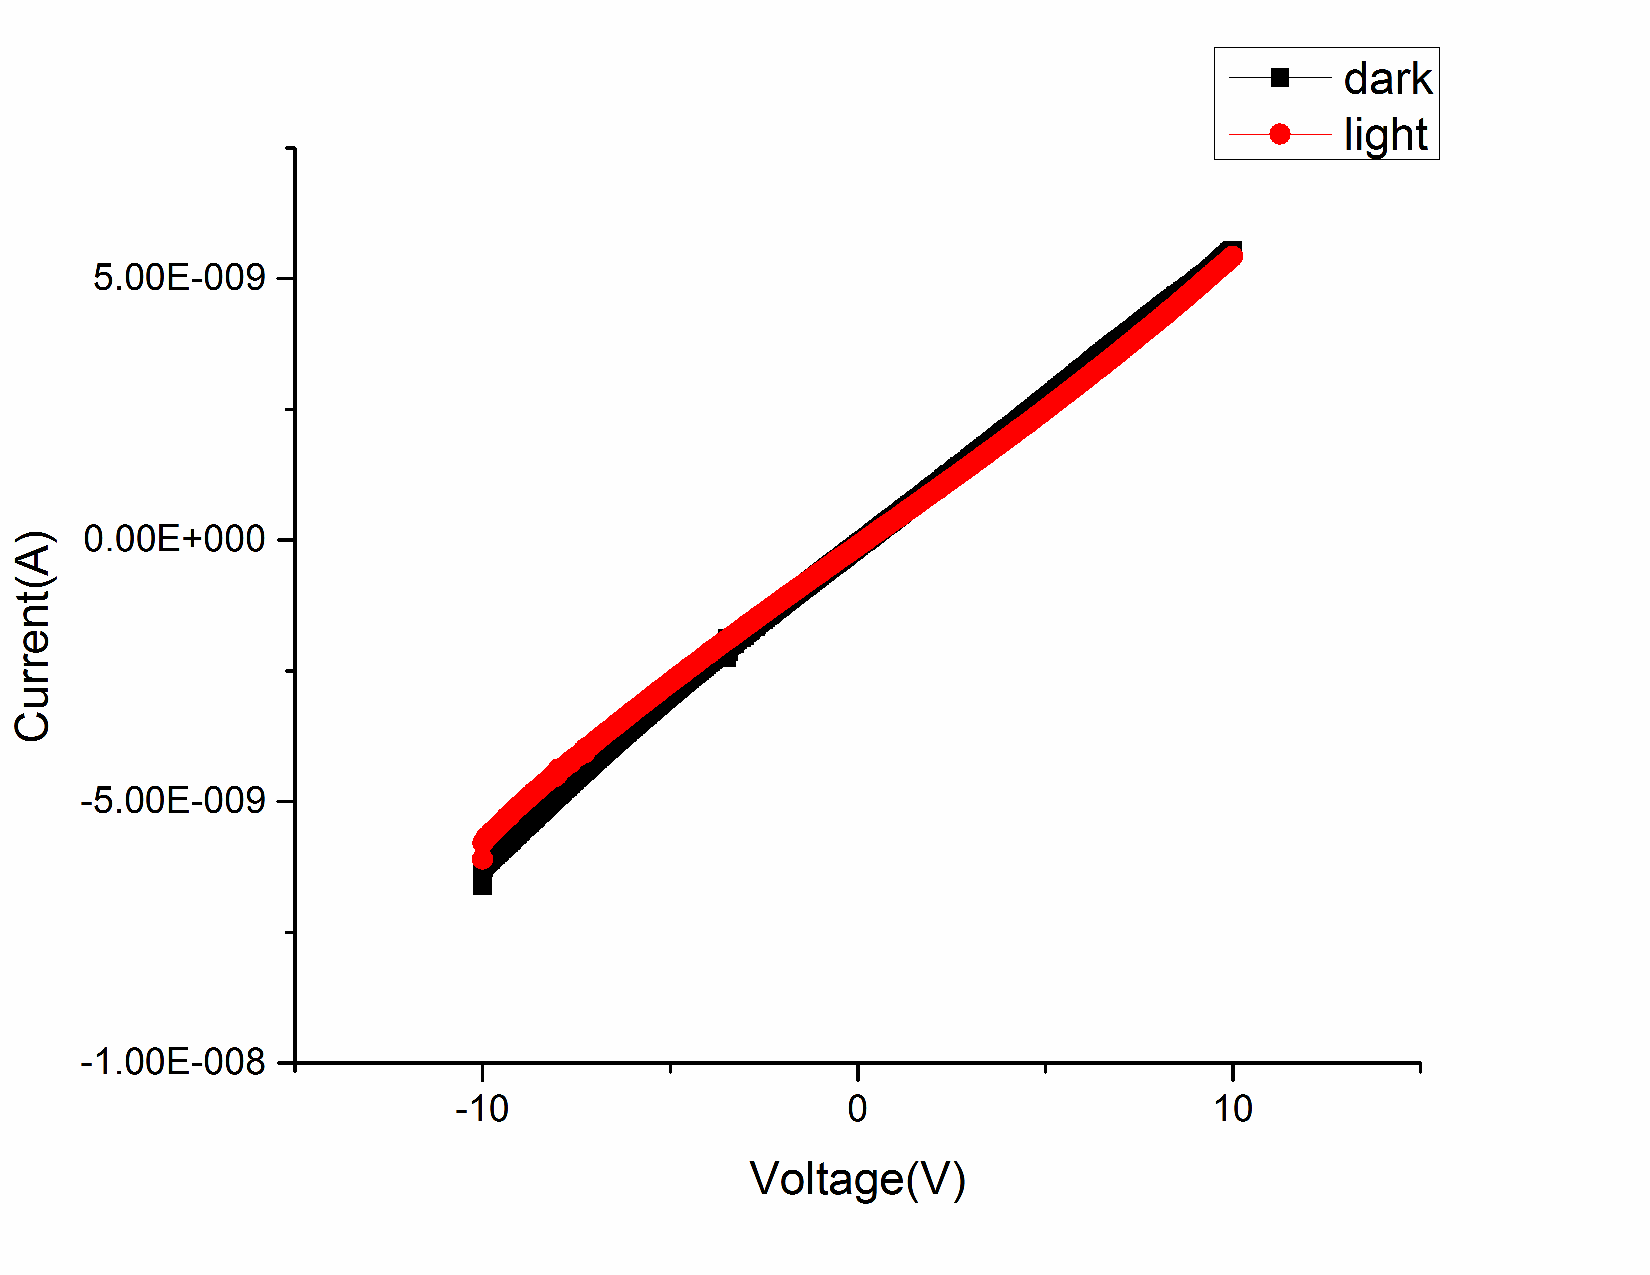
\includegraphics[width=\textwidth]{pictures/Data/CSNWIV_light}
  \label{CSNWIV_light}
\end{figure}

\section{Absorption Enhancement} \label{X-ray}

\begin{figure}
  \caption{Reflective Measurement for Bulk GaAs and Si}
  \centering
  \includegraphics[width=\textwidth]{pictures/Data/reflecbulk}
  \label{reflecbulk}
\end{figure}

\begin{figure}
  \caption{Reflective Measurement for Core-Shell Nanowires Grown on Bulk GaAs and Si}
  \centering
  \includegraphics[width=\textwidth]{pictures/Data/reflectCSNW}
  \label{reflectCSNW}
\end{figure}

\section{Emission Enhancement} \label{Dust_data}

\begin{figure}
  \caption{Photoluminescence Experiment for Core-Shell Nanowires Grown on Bulk GaAs and Si}
  \centering
  \includegraphics[width=\textwidth]{pictures/Data/PL}
  \label{PL}
\end{figure}

\section{Lasing} \label{BH_data}

\begin{figure}
  \caption{Photoluminescence Experiment Demonstrated Lasing Behavior for Core-Shell Nanowires Grown on Bulk GaAs and Si}
  \centering
  \includegraphics[width=\textwidth]{pictures/Data/lasing}
  \label{lasing}
\end{figure}

  
  %CHAPTER: Light Management
  \chapter{Light confinement in sub-wavelength nano-structure} \label{LM}


\section{Light and Nanowire} \label{corrections}


\subsection{Leaky Mode Resonance}
\label{sec:hydrogen}
Interaction of light with a dielectric or metallic cylindrical medium is analyzed by solving Maxwell's equations with the appropriate boundary conditions in the classical waveguide theory [80] which leads to highly confined modes in optical fibers and microscale dielectric resonators. In an infinitely long cylinder, even at deep sub-wavelength diameters this results in a “characteristic equation” the solution to which are the transverse magnetic (TM) and transverse electric (TE) resonant modes. We can define the electromagnetic modes of localized resonators as time-harmonic solutions of the form  to the source-free Maxwell equations. This solution shows that the longitudinal field component distributes outside the NW, and is in resonance with the natural modes, such as TE11, TM02, etc., supported by the NW. These modes have been termed leaky-mode resonances (LMR) [81, 82], and provide an intuitive tool to facilitate the understanding and optimization of the resonance effect in such nano-structures. 
We replicate these results using MEEP, a widely used open-source finite-difference time-domain (FDTD) simulation package [83], to identify how light is confined in an infinitely long GaAs nanowire. The top row of Fig. 1 shows several configurations of TM LMR modes for a NW with diameter of 220nm, with excitation single wavelength light being incident parallel to the NW axis. The blue and red color codes represent the polarization of the electric fields. The TE modes are primarily identical to the TM modes shown here with the electric and magnetic fields exchanged. If the light is incident with an arbitrary angle, then so-called hybrid HE and EH leaky modes will be excited instead of the pure TE or TM mode.  The bottom row of Fig. 1 shows the directional energy flux density of the electromagnetic field, the Poynting vector, at different time frames with light being incident perpendicular to the NW axis from the right side. The light is seen to propagate from the right and then mostly remain confined at the left part of the cylinder. It is notable that in either case the light energy is spatially distributed along the cross section of the wire but, as expected from a 2D treatment does not vary axially. Figure 1 demonstrates that the LMR can gently confine light within subwavelength semiconductor nano-structures, similar to the intuitive ray-optics picture of multiple total internal reflections from the periphery of the cylinder. As shown by in Ref. [81], these LMRs depend on the radius and the height of the dielectric, which allows ‘light engineering’ of the nanowires so as to increase its absorption efficiency at pre-determined wavelength, e.g., to maximize absorption of sunlight spectrum for  higher efficiency solar cells, or to radiate as optical antennas. 

\subsection{Whispering Gallery Modes}
\label{sec:host}
Infinitely long cylindrical or hexagonal NW structures can also support Whispering Gallery (WG) modes [78, 79, 84-90]. To calculate the resonant WGMs, Maxwell’s equations have to be solved numerically [91] taking into consideration the spectral dependence of the material of interest’s index of refraction. However, we can deduce a simple plane-wave model from theoretical derivations, and the relationship between resonance wavelength λ and the corresponding mode serial number N can be obtained [92]. The WG modes can also reflect and confine light in the (subwavelength) nanostructure by total internal reflection from the curvature of the structure boundaries. However, a light wave can interfere with itself only when having completed one full circulation within the resonator, which means only the light with one or multiple wavelengths are allowed to perform multiple circulations generating a standing wave. Figure 2 from reference 85 shows near-field intensity patterns of low-order TM polarized hexagonal WGMs for n=1 and refractive index =2.1. Each mode pattern is labeled by its respective mode number m (lower right number) and its symmetry class (upper right symbol). 
For comparison, four mode patterns of the circular cavity are given in the upper left and lower right together with their angular mode number. We again observe the radial spatial dependence of light intensity. Furthermore, the low order WG modes of hexagonal NWs are essentially similar to the cylindrical ones, but for higher order modes additional features will arise on the facets of the hexagonal NWs [85]. Simulation results also show little difference between WG mode and Leaky modes in lower order modes for both hexagonal and cylindrical structures. As with the LMR, the resonant WG modes have been used as the basis for a precise theoretical explanation of the enhanced optical behavior of hexagonal NWs, such as enhanced light absorption [81, 93-96] and emission [78, 97-99]. Furthermore, these numerical solutions have lead to reproduction of experimental resonance spectra, e.g., polarization-resolved micro-photoluminescence (µ-PL) and cathodeluminescence (CL) spectroscopy. 
\subsection{Fabry-Perot Resonant Mode}
The above analysis and results apply to long structures, hence, provide two-dimensional radial modes, independent of the NW axis. However, light confinement has strong axial dependence, necessitating three-dimensional analysis of the cavity modes. FDTD simulation in 3D are used to identify the axial dependence of resonant modes in these nano-structures, revealing modes which are volumetric in nature.
Fabry-Perot (FP) modes have been analyzed for sub-microcavity, or nano-cavity, NWs with cylindrical or hexagonal structures, specifically in order to determine the axial dependence of the resonance modes [100]. At least two mirrors are needed to construct the reflection structure inside the cavity, whether they are the top and bottom ends, i.e., the air and substrate interfaces with the nanowire, or any of the two opposite facets along the nanowire axis. For subwavelength structures, the longitudinal WG modes have high scattering losses due to diffraction, and axial FP waveguide modes will dominate [90]. However, due to small difference of the refractive index between the substrate and the nanowire dielectric, the existence of the FP mode will only be valid if the nanowire has relatively large radii, e.g., larger than 200 nm [101]. Under these conditions, besides the top and bottom ends, the lateral facets of nanowire can also be treated as two parallel slabs, and with the dielectric in between, it can support the FP mode with mode spacing inversely related to the nanowire length. An application of this analysis is in the design of NW lasers, since the optical cavity modes are observed at threshold for lasing, and have been investigated for both optical and electrical pumped cases [102, 103]. As a results the FP resonance mode based nanoscale lasers are not only capable of covering a wide spectral regions, but can also can be integrated as single or multi-color laser source arrays in silicon based photonic integrated circuit or microelectronic devices [102,103]. However, the FP modes supported by the nano-cavity structure have relatively small quality factor due to the small difference of the refractive indices of the substrate and the NWs. In order to address this issue,  Bragg gratings can be produced at the NW ends, alternatively, NWs can be placed on metal substrates in order to increase the FP resonance peak intensity by more than one order of magnitude compared to those on Si substrates [104].
\subsection{Helical Resonance Modes}
Nano needles of III-V material grown on heterogeneous substrates are optoelectronic devices which have shown interesting optical behavior, including lasing, at room temperature [105]. Figure 3 (A) shows SEM image of a nano-laser grown on silicon substrate that has subwavelength dimensions on all sides. Analysis of light propagation introduced by shows that unlike the traditional WG mode that lack vertical structure, there is net propagation in axial direction in these structures which leads to  volumetric resonant modes which are termed helical mode resonances [105]. The schematic Fig. 3(B) suggests a helical ray path with nearly total internal reflection at the nanopillar-silicon interface due to the glancing angle of incidence from the hexagonal facets of the nano-laser shown in Fig. 3(A). As such, the faceted shape of the structure affects the optical cavity properties. FDTD-simulated field profile shows a hexagonal WG-like mode pattern  in the transverseplane as in Fig. 3 (C), which arises from strong azimuthal components of helical modes. Figure 3 (D) shows first-order  and higher-order standing waves’ axial variation. The radial mode number (first number, m) describes the transverse field pattern for WG modes, and the axial mode number (second number, n) describes the axial standing wave as is the case for Fabry-Perot resonances. It is seen that light or optical field can be well confined in the nanostructure even with low index contrast at the dielectric interface thus producing the nano-resonators needed for lasing. Although the quality (Q) factors of such nanostructure are usually not large, these helically propagating cavity modes, provide an optical feedback mechanism without the sophisticated mirror structures of the vertical cavity surface emitting lasers (VCSEL’s). Additionally, since the nanowires are heteroepitaxially grown on different substrates, they enable heterogeneous integration of photonic emitters and silicon based computational circuitry.  Whereas traditional FP modes are inhibited by the interface between semiconductor nanostructure and the silicon substrate, such unique optical structures have been proposed as an avenue for engineering and integrating on-chip nanophotonic devices. 

\section{Volumetric Modes} \label{sed}
The diameter of the nanostructures which can support the helical resonance modes is near the Rayleigh limit, around the boundary of the validity of ray-optics. FDTD analysis can be applied to deeper subwavelength structure in order to identify the cavity modes which are by nature volumetric, i.e., axially dependent.  Figure 4 shows simulation results for various diameters of hexagonal structure of 1 m length.  Incident radiation with 532 nm wavelength is nearly parallel to the wire axis and different modes are displayed for different radii. Top row shows radial spatial dependence at the middle of the wire axis, and the bottom row shows the axial dependence. Top row results are similar to Figures 1-2, and the bottom row shows that the light can be confined in volumetric resonance mode in both transverse plane and longitudinal plane even with sub-wavelength diameter of these hexagonal NWs. Unlike helical modes, the explanation of resonance  need not rely on an intuitive ray-optics description based on the grazing angle of incident light, but shows similar results in how the deep subwavelength structures can confine the light and produce a resonant cavity without having sophisticated mirrors at the end facets. In this respect nano-cavities of as-grown nanowires outperform microcavities of VCSELs.
\subsection{Nanocavity Geometry Dipendence}

\subsection{Light Engineering of Nanocavities}
Dependence of the resonant modes on the cavity geometry offers an important degree of freedom to engineer a cavity for particular optical properties. Figure 6 shows the dependence of three volumetric TM resonant modes’ excitation wavelengths with radius. In this spectral range, only lower TM modes can be excited with smaller radii, e.g., r = 40 nm and 60 nm, however, as the radius increases, higher order modes can be excited, and the optical power corresponding to the lower order modes will be reduced. We observe redshift of these volumetric TM modes with increasing NW radius. Also, the wavelength variation of TM1n mode is much larger compared to TM2n and TM3n modes. These observations demonstrate the feasibility to engineer the volumetric mode at certain wavelength, i.e., allow us to optimize absorption or emission at a desired frequency or certain incident optical power  by controlling the radius and/or length of a NW thus providing the ability to engineer the absorption spectrum in order to match desired properties.

iThe dependence of the resonant modes on NW radius also suggests the interesting possibility of having tapered structures which can support more than one resonant mode, thus be able to optimize the spectrum of interest.  The metalorganic vapor phase epitaxy (MOVPE) or vapor liquid solid (VLS) growth methods are readily capable of forming nanowires with tapered sidewalls. The resultant cavity, however, does not support the superposition of the modes present in cylindrical structures of the same diameter; in fact tapered sidewalls have been identified as the primary loss mechanism for these sub-wavelength cavities.  The effect of  tapering has been studied for  nanopillars that were grown on a silicon substrate with average 5° angles between opposite sidewalls; vertical field profiles for ,  and  modes are shown in Fig. 7 [105]. The modes are primarily confined at the base, and become less resonant as they propagate upwards with decreasing of the radius at top. Higher-order axial modes generally have lower quality factor. Physically, the stronger Fabry-Perot characteristic of higher-order axial modes means that their effective longitudinal wave-vector components become stronger, causing larger penetration and loss into the substrate. Nevertheless, from a different perspective, multi-mode resonances can be achieved within certain wavelength range by controlling the tapering angle in order to form small varying radius along the nanostructure axial direction. One can also red- or blue-shift the resonance peaks, since these volumetric resonance modes are dependent on transverse dimensions. Thus, intentioned tapering offers an alternative way to engineering the multi-mode resonances and finer tunability of these resonance peaks.

%\subsubsection{\civ-dependent Mean} \label{CIV SED}




  
  %CHAPTER: Electronic Density Distribution
  \chapter{Reduced Electronic Density Distribution} \label{ED}

A heterojuntion is basically a p-n junction in a semiconductor between
materials of different composition. Normal junctions are between p and n type
versions of the same material. But in this case we refer to a juntion formed
betewen two group III-arsenide usually a GaAs/AlAs interface or a GaAs/AlGaAs
interface. Since they are two differnt materials, the band structure is
discontinuous from one material to the other and the band alignment across the
interface is typically of type I, i.e. the band gap of the lower bandgap
material is positioned energetically within the bandgap of the wider bandgap
semiconductor.

Polarization fields 
The usual growth direction for hexagonal III-V materials is
along the polar [0001] axis, for which the crystal lacks inversion symeetry.
This will result in the formation of polarization fields. There are two kinds
of polarization fields. They are spontaneous polarization (SP) and
Piezoelectric polarization (PZ).  The spontaneous polarization exists in polar
semiconductors with a Wurzite or lower symmetry crystal structure and is
related to the deviation of the crystal lattice parameters from the ideal
values for the structure, thereby creating molecular dipoles in the material
building a polarization field just like that formed in ferroelectrics. This
field has a fixed direction along the [0001] c-axis in the Wurtzite lattice.
Therefore the field resulting from spontaneous polarization will point along
the growth direction and this maximizes pontaneous polarization effect in these
systems and renders the problem effectively one-dimensional.  

The other type of polarization field, the piezoelectric polarization occurs due
to the presence of strain in the system. When two layers are joined together to
form a heterojunction, the difference in the lattice constant between the two
materials will lead to a strain . This strain also occurs due tot he difference
in the thermal expansion coefficients in the the layers during cool down after
growth. This leads to elastic strain in the layers. 

\section{Self-consistent Poisson-Schrodinger Solver} \label{sec:model}

The study of energy band structures of heterostructures needs a detailed
knowledge of optical and transport properties of the heterostructures. These
properties can be found by solving sefl-consistently Poisson's and
Schrodinger's equations for the elctron wave functions.

The finite difference method (FDM) is a simple and efficient method for solving
ordinary differential equations (ODEs) in problem regions with simple
boundaries. FDM can be used to solve for the Schrodinger equation. The method
requires the construction of a mesh defining local coordinate surfaces. For
each node of this mesh, the unknown function values are found, replacing the
differntial equations by difference equations. These values gives the vector
solution for $\phi$ and a matric formulation if the Schrodinger equation.
where A is the matrix operator and $\lamda$ the energy eigenvalues. Usually a
uniform mesh size is selected but this means that this method is not effective.
Need a small mesh when the wavefunction is changing rapidly and a large mesh
during a slow change in the wavefunction for the ideal speed. Moreover, careful
calculations are also required at the juntion of two different mesh sizes and
destroying the symmetry of the matrix A, making it more difficult to calculate. 
%\subsection{What Reddening Law Fits Better?}\label{sec:DIC}


\section{Electronic Distribution in Nanowires} \label{sec:spectra}

Figure 8 (C) shows the FDTD-simulated electric field density of a hexagonal
nanowire at y cross section (top) and x cross section (bottom). The photon
energy of this mode shown as the insets of Fig. 8(C) is concentrated primarily
along the 6 corners and secondarily along the facets with little light in the
3D core of GaAs. Hence, we suggest that the fortuitous spatial overlap of the
resonant optical modes on reduced dimensional electronic wavefunctions plays a
significant role in the remarkable optoelectronic properties of core-shell
nanowires. Restated, the superposition of the photon modes  on reduced
electronic states that form on the facets and vortices of the hexagonal CSNWs
strongly enhances both upward and downward transition rates.  Thus, the reduced
dimensionality transition rate distinguishes the core-shell nanostructure from
the optically equivalent structures of Fig. 6 due to its significantly modified
rate management. These nanostructures are not only excellent optical cavities,
but despite their large size also provide the right reduced dimensional
electronic structures which enhance optoelectronic interactions.  It should be
noted the present analysis is for direct optical transitions; although it can
be extended to incorporate k-vector changes as in phonon scattering, other
important factors such as many-body interactions need to be included in a
comprehensive analysis.

\subsection{Cylindrical Core-Shell Nanowire}

\subsection{Hexagonal Core-shell Nanowire} \label{sec:indv_lines}

\begin{figure}
  \caption{One Dimensional Electron Charge with band bending}
  \centering
  \includegraphics[width=\textwidth]{pictures/ED/1DCharge}
  \label{1DCharge}
\end{figure}

\begin{figure}
  \caption{Two Dimensional Electron Charge with band bending}
  \centering
  \includegraphics[width=\textwidth]{pictures/ED/2DCharge}
  \label{2DCharge}
\end{figure}

\begin{figure}
  \caption{Three Dimensional Electron Charge with band bending}
  \centering
  \includegraphics[width=\textwidth]{pictures/ED/3DCharge}
  \label{3DCharge}
\end{figure}

\begin{figure}
  \caption{Photon Charge Distribution}
  \centering
  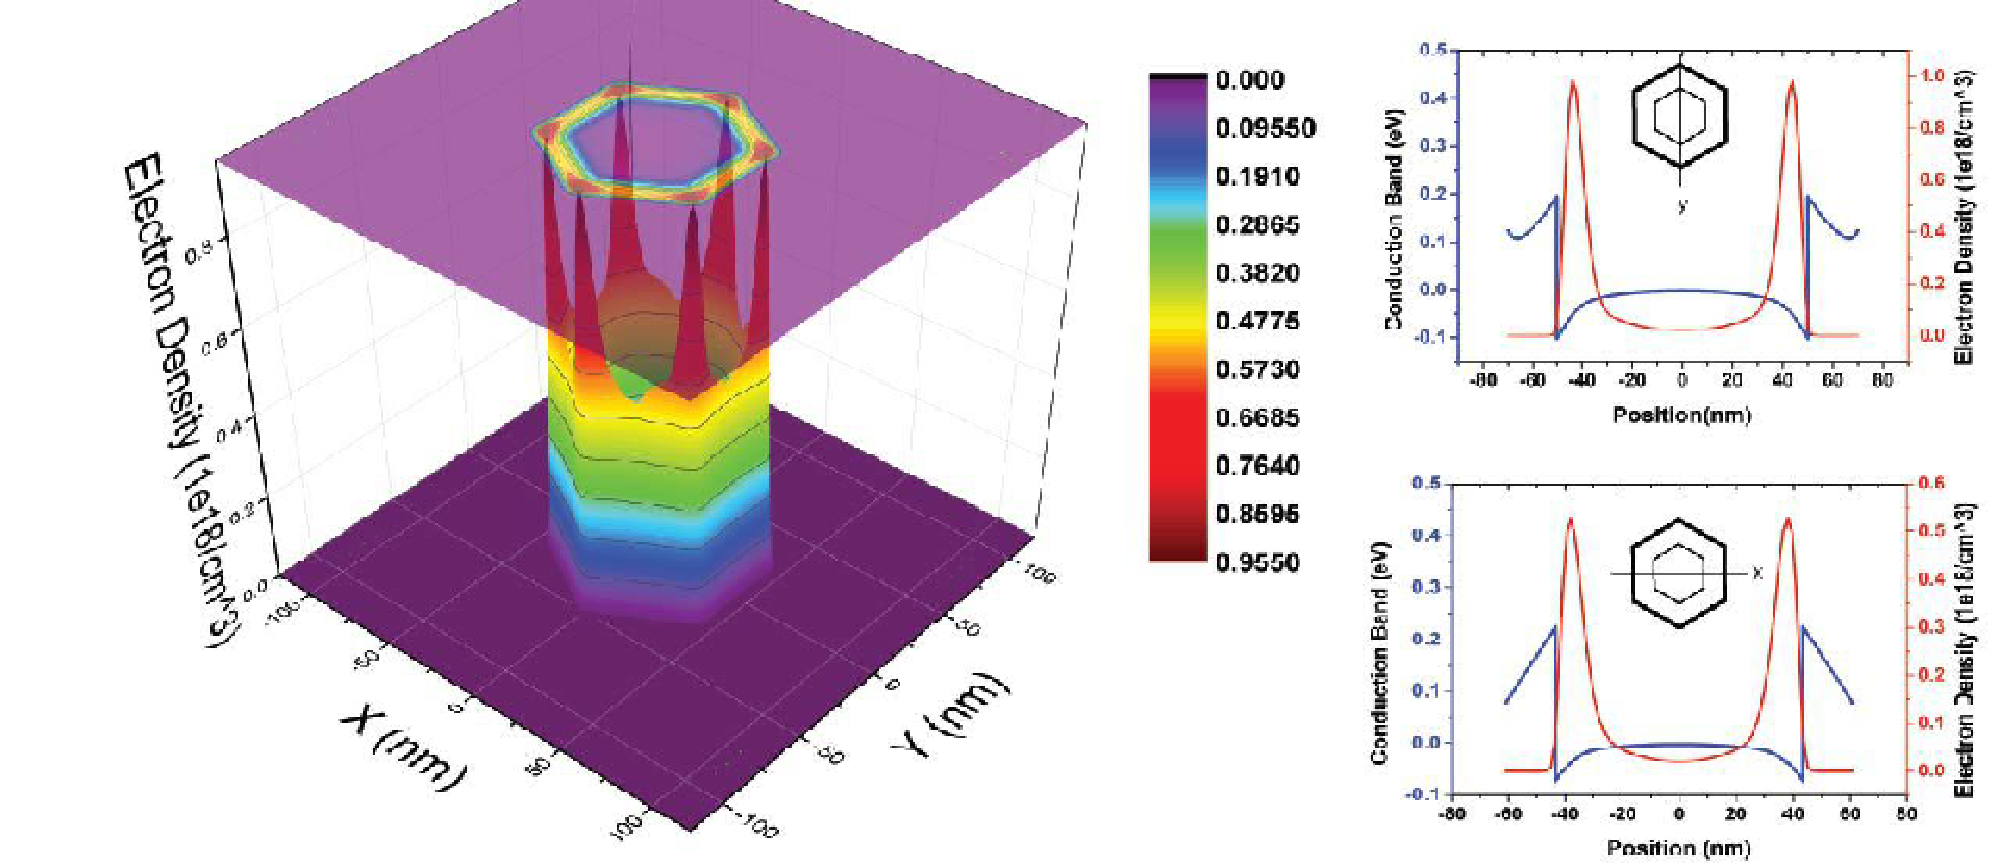
\includegraphics[width=\textwidth]{pictures/ED/Photoncharge}
  \label{PhotonCharge}
\end{figure}

\section{Conclusions} \label{sec:conclusions}


  
  %CHAPTER: Rate Management
  \chapter{Dimensional Dependence of Optical Transition Rates} \label{RM}
 
\section{Time-dependent Perturbation Theory} \label{dust_seds}

\subsection{} \label{dust_corrections}

%\subsection{A Uniform Sample}
%\subsection{\ltwofive\ and \bctwofive\ Distributions} \label{l_bc_dust}
%\subsection{Extinction Corrected SEDs} \label{l_bc_dust}

\section{Upward and Downward Transition Rates} \label{mbh_seds}

\section{Contributing Factors} \label{BH_conclusions}
\subsection{Overlap Integral}
\subsection{Oscillator Strength}
\subsection{Joint Optical Density of States}
The preceding theory of gain involving Fermi's Golden Rule considers each electron in isolation as it interacts with the electromagnetic field. In other words, we have used a single-particle theory to obtain the gain spectrum. In reality, there is a large density of both electrons and holes present in the system. The mutual interactions between these particles are generally referred to as many-body effects. These effects included lineshape broadening, which is related to collisions between particles and/or phonons in the crystal. In addition to this important effect, there are two other significant consequences of many-body effects: exciton states and bandgap shrinkage. Exciton states exsit primarily at low carrier densityies and low temperatures, where bandgap shrinkage becomes noticeable at high carrier densities.

Under conditions of low carrier density and low temperature, it is possible for an electron and hole to orbit each othere for an extended period of time, forming what is referred to as an exciton pair. Such exciton pairs have a binding energy associated with them that is euqal to the energy required to separate the electron and hole. As a rsult, electrons that are elevated from the valence band to one of these exciton states will absorb radiation at energies equal to the bandgap less the binding energy (the bandgap will appear to be red-shifted). More significatnly however, the overlap integral ( and hence the matrix element ) of these two-particle states can be quite large. As a result, band-to-exciton transitions tend to dominate the absorption spectrum. However, exciton states are limited to states near $k = 0$, and hence band-to-exciton transitions are clustered at the band edge (or subbabdn edge). The overall effect is the qppearance of very strong absorption peaks near the subband edges in quantum-well materials, and near the band edge in bulk material.
Exciton absorption peaks are clearly visible in quantum wells at room temperature for a typical GaAs QW. The first two steps in the "staircase" absorption spectrum predicted from the density of states. However, the exciton peaks riding on top of the steps, particularly the n = 1 peaks, dominate the absorption spectrum. Each observed exciton peak corresponds to one of the subband transitions.

The second many-body effect occurs at high carrier densities, where the charges actually screen out the atomic attactive forces. With a weaker effective atomic potential, the single-atom electron wavefunctions of interest become less localized and the nearest-neighbor electron everlap becomes higher.  The large overlap increases the width of the energy bands ($\delta{E}$ is larger), reducing the gap between bands. Although this description is only qualitative, it does reveal that the bandgap should shrink with increasing carrier density.
It can also be argued theoretically that the badgap shrinkage is inversely related to the average spacing between carriers, or (the closer the carriers are, the more their own Coulomb potentials screen out the atomic potential). In bulk material, the average volume occupied by one carrier is inversely related to the carrier density. 
The net effect of bandgap shrinkage is that as carrier density increases, the entire gain spectrum redshifts by a noticeable amount. In principle, the shift is accompanied by a slight distortion. (i.e, reshaping and enhancement) of the spectrum.


  %CHAPTER: Laser Threshold Calculation
  \chapter{Modeling Lasing Threshold} \label{LT}


\section{History of Semiconductor Lasers} \label{corrections} As we know,
semiconductor lasers are important optoelectric devices ofr optical
communication systems. They are essential components for building optical
communication systems. There are intensive research results and achievements
from beginning.  In 1917, Einstein predicted the existence of spontaneous and
stimulated emission by which an atom can emit radiation. The first
semiconductor lasers were fabricated in 1962 using homojuncations. These lasers
had high threshold current density ( 19000/A/cm2 ) and operated at cryogenic
temperatures.  The concept of heterojuntion semiconductor lasers was realized
in 1969~1970 with a low threshold current density (1600 A/cm2) operating at
room temperature. These double-heterostructure diode lasers provide both
carrier and optical confinements, which imporve the efficiency for stimulated
emission.  The concept of quantum well structures for semicondcutor lasers was
proposed and realized experimentally in the late 1970s. The threshold current
density was reduced to about 500 A/cm, which improved the laser performance
significantly.

\section{Principle of Semiconductor Lasers} \label{corrections}

As we know, the semiconductor laser (or laser diode) in its simplest form is a
p-n junction of a single crystal of semiconductor material arranged in a
cavity, as shown in . The type and configuration of the material used to
determine the optical characteristics of the laser diode emission. Like others
in various oscillators or wave sources, the fundamental elements in the
semiconductor lasers are the following three elements: semiconductor band
structure (population inversion to provide gain mechanism), current injection
and P-N junction ( external pumping to make gain sustainable) and reflector of
cavity (feedback to provide coherence). The most common semiconductor lasers
are including Fabry-Perot(FP) or distributed feedback (DFB)/distributed Bragg
reflector (DBR) 

\subsection{Absorption of Light}

The light and matter interaction includes absorption, spontaneous emission and
stimulated emission, we first discuss the absorption of light by introducing
the absorption coeffiecient. This is the absorption rate without considering
the occupation factors.

Based on the following equations for different dimensionality.


\begin{equation}
\begin{aligned}
    \alpha_{3D}(\hbar\omega)= & C_0{|\hat{e}\cdot\bf{p}_{cv}|^2}(f_v-f_c)\\
    & \frac{1}{2\pi^2}(\frac{2m_r^\ast}{\hbar^2})^{3/_2}(\hbar\omega-E_g)^{1/_2},\\
    & C_0=\frac{\pi{e^2}}{n_r\epsilon_0{c}{m_0^2}\omega},
\end{aligned}
\label{eq:two}
\end{equation}

\begin{eqnarray}
\begin{aligned}
& \alpha_{2D}(\hbar\omega)=C_0{|\hat{e}\cdot\bf{p}_{cv}|^2}\frac{m_r^\ast}{\pi\hbar^2{L_z}},
\\
& \alpha_{1D}(\hbar\omega)=C_0{|\hat{e}\cdot\bf{p}_{cv}|^2}\frac{{(m_r^\ast)}^{3/_2}}{\pi\hbar{m_e^\ast}{L_x}{L_y}}\frac{1}{\sqrt{(\hbar\omega-E_g)}},
\end{aligned}
\label{eq:five}
\end{eqnarray}

The split plots of absorption coefficient for different dimensionality as in
Fig.~\ref{absrate_split}. Noted the unique shapes of density of states.

\begin{figure}
  \caption{Absorption Coefficient versus Photon Energy for 1D 2D and 3D with split plot}
  \centering
  \includegraphics[width=\textwidth]{pictures/LT/absrate_split}
  \label{absrate_split}
\end{figure}

Then the overlay plot with multiple y axis as in Fig.~\ref{absrate_overlay} and
the different scales indicating the enhancement factor for 1D is 35(need to be
verified) compared to 3D.

\begin{figure}
  \caption{Absorption Coefficient versus Photon Energy for 1D 2D and 3D}
  \centering
  \includegraphics[width=\textwidth]{pictures/LT/absrate_overlay}
  \label{absrate_overlay}
\end{figure}

\subsection{Optical Gain}

Following the treatments of Appendix 3, we can derive the gain spectrum for 3D,
2D and 1D with consideration of occupation factor by calculating the Fermi
levels.

With decreasing dimensionality of the active region of an injection laser, the
density of states and gain spectra become narrower, which leads to a decrease
in the number of states to be filled to make the active region transparent
(zero population inversion and zero gain) and to achieve lasing (gain equal to
loss). Consequently, the transparency current (or inversion current, i.e., the
injection current at which the population inversion is zero) and the threshold
current (injection current at which the gain is equal to the loss and lasing
begins) decrease and their temperature dependences become weaker. The decrease
in the threshold current and increase in its temperature stability reflect one
fo the main areas of development and improvement of injection lasers. Owing to
the continuous nature of the carrier spectrum within the allowed subbands, the
use of QWs or QURs as active medium for optical transitions can only
quantitatively improve the parameters of devices based on them compared with
devices with a bulk active region. 

Among the advantages of QD lasers over the presently used QW lasers are their
narrower gain spectra, much lower threshold currents, and ultrahigh temperature
stability, as well as the wider possibilities for controlling their lasing
wavelength.

All the parameters for rate quations analysis in table~\ref{tab:rate_eq}.

\setlength{\tabcolsep}{4pt}

\begin{deluxetable}{ll}
\tabletypesize{\footnotesize}
\tablewidth{0pt}

\tablecaption{Quasar Catalog Format \label{data_table}}
\tablehead{\colhead{Column} & \colhead{Description}}
\startdata
1   &   Previously published name\\
2   &   Right ascension in decimal degrees (J2000)\\
3   &   Declination in decimal degrees (J2000)\\
4   &   Redshift       \\
5   &    BEST SDSS {\em u} band PSF magnitude\\
6   &    Error in {\em u} magnitude\\
7   &    BEST SDSS {\em g} band PSF magnitude\\
8   &    Error in {\em g} magnitude  \\
9   &    BEST SDSS {\em r} band PSF magnitude\\
10  &    Error in {\em r} magnitude  \\
\enddata
\tablecomments{This table is available in its entirety in a machine-readable form in the journal publication \citet{Krawczyk:2013}.
A portion is shown here for guidance regarding its form and content.}
\end{deluxetable}

\begin{eqnarray}
\begin{aligned}
  & g_{3D}(\xi)=\frac{\sqrt{2}e^2{m_r^\ast}^{3/2}{p_{cv}^2}}{3{\pi}n_r\epsilon_0{m_0}^2C{\hbar^2}\xi}{\sqrt{(\xi-\xi_g)}}(f_n(\xi_2)-f_p(\xi_1)),
\\
& g_{2D}(\xi)=\frac{e^2{m_r^\ast}{p_{cv}^2}}{3{n_r}\epsilon_0{m_0}^2C{\hbar}L_z\xi}(f_n(\xi_2)-f_p(\xi_1)),
\\
& g_{1D}(\xi)=\frac{e^2{m_r^\ast}^{3/2}{p_{cv}^2}}{3{n_r}\epsilon_0{m_0}^2C\xi{L_x}{L_y}}\frac{1}{\sqrt{(\xi-\xi_g)}}(f_n(\xi_2)-f_p(\xi_1)),
\end{aligned}
\label{eq:five}
\end{eqnarray}

Now we can plot the gain spectrum respect to photon energy for 3D, 2D and 1D in
the figure below. As we can see, the gain spectrums follow the unique shapes of
density of states. The fourth figure is the maximum gain versus electron
carrier concentration varing from $3\times10^{18} (cm^{-3})$ to
$3\times10^{19}(cm^{-3})$. Using parameters $N_{tr} = 2\times10^{18} cm^{-3}$,
$N_{s} = 4\times10^{18} cm^{-3}$, and $g_0 = 6.11\times10^{5} cm^{-1}$, we fit
the curve in Fig.~\ref{gainspectrum} to build a logarithmic gain model of the
form for 3D case:

\begin{equation}
  g(N) = g_0\ln\left(\frac{N+N_s}{N_{tr}+ N_s}\right)
\end{equation}

where $N_s$ is a shift to force the natural logrithm to be finite at $N = 0$
such that the gain equals the umpumped absorption due to the band-to-band
transitions, $N_{tr}$ is the transparency carrier density, and $g_0$ is the
gain coefficient. $N_{tr}$ and $g_0$ will be different for different
dimensionality.

\begin{figure}
  \caption{Gain Coefficient versus Photon Energy for 1D 2D and 3D}
  \centering
  \includegraphics[width=\textwidth]{pictures/LT/gainspectrum}
  \label{gainspectrum}
\end{figure}

\begin{figure}
  \caption{Gain Model Fitting}
  \centering
  \includegraphics[width=\textwidth]{pictures/LT/gainModelFit_Anoted}
  \label{gainModelFit_Anoted}
\end{figure}

After fitting the curve in Fig.~\ref{gainModelFit_Anoted}, we can calculate the
threshold carrier density is $N_{th} = 4.533\times10^{18} cm^{-3}$. Then
plotting the spontaneous emission rate with respect to the threshold carrier
density $N_{th}$ for 3D, 2D and 1D as following: 

\begin{eqnarray}
\begin{aligned}
& r_{3D}^{\mathrm{spon}}(\xi)=\frac{n_re^2\xi{p_{cv}^2}}{{\pi}\epsilon_0{m_0}^2C^3{\hbar^2}}\frac{{m_r^\ast}^{3/2}}{2\pi^2\hbar^3}{\sqrt{(\xi-\xi_g)}}f_n(\xi_2)(1-f_p(\xi_1)),
\\
& r_{2D}^{\mathrm{spon}}(\xi)=\frac{n_re^2\xi{p_{cv}^2}}{{\pi}\epsilon_0{m_0}^2C^3{\hbar^2}}\frac{{m_r^\ast}}{\pi\hbar^2L_z}f_n(\xi_2)(1-f_p(\xi_1)),
\\
& r_{1D}^{\mathrm{spon}}(\xi)=\frac{n_re^2\xi{p_{cv}^2}}{{\pi}\epsilon_0{m_0}^2C^3{\hbar^2}}\frac{{m_r^\ast}^{3/2}}{\pi\hbar{m_e^\ast}L_xL_y}\frac{1}{\sqrt{(\xi-\xi_g)}}f_n(\xi_2)(1-f_p(\xi_1)),
\end{aligned}
\label{eq:six}
\end{eqnarray}

\begin{figure}
  \caption{Spontaneous Emission Rate versus Photon Energy for 1D 2D and 3D}
  \centering
  \includegraphics[width=\textwidth]{pictures/LT/sponrate}
  \label{sponrate}
\end{figure}

Integraing over all the photn energy spectrum, we have $R_{sp} =
\int_{\xi}r_{sp}d{\xi}$ for different dimensionality, then the threshold
current density can be simply caluclated as: $J_{th}= qdR_{sp}|_{N_{th}}$ and
plotted in the fourth part of Fig.~\ref{sponrate}. The threshold current for 3D
is $2.62\times10^{27} (A/cm^2)$, 2D is $2.42\times10^{10} (A/cm^2)$, and 1D
case is $4.73\times10^{6} (A/cm^2)$. The threshold current density needed for
lower-dimensional structure is greatly reduced.

Next, we can do dynamic analysis of laser modal and replace the threshold
current density to threshold pumping power. And verify the result with the
experimental data.

\subsection{Feedback and Laser Threshold}
\section{Types of semiconductor Lasers} \label{corrections}
\subsection{Fabry-Perot Semiconductor Lasers}

The Fabry-Perot(FP) laser is conceptually just an LED with a pair of end
mirrors or facets. The mirrors are needed to create the right conditions for
lasing to occur. The lasing medium can only amplify (undergo stimulated
emission) over a fairly narrow range because of the characteristics of the
material it is made from . A typical gain curve is illustrated on the
left-hand. 

\subsection{Grating-Based semiconductor Lasers}
\subsection{Vertical-Cavity Surface-Emitting Lasers}

As seen, light in the VCSEL propagates vertically with DBR mirrors as the
nature of the manufacturing process, the entire round-trip of the VCSEL is much
shorter than that of with the edge-emitting lasers. It leads to high
reflectivity ( around 99.9$\%$) of DBR mirrors, in which the large number of
layers are required.

One of features related to the VCSELs is the longitudianl modal stability due
to its short cavity length (around order of the wavelength). A

\subsection{Grating Surface-Emitting Lasers}
\section{Characteristics of Semiconductor Lasers} \label{corrections}

In order to understand their operation, it is necessary to know some basic
performance parameters or important features of semiconductor lasers.

\section{Basic Requrement for Design of Semiconductor Lasers} \label{corrections}
\subsection{Spectral width and Linewidth}

FP semiconductor lasers produce a range of wavelengths. This range of
wavelengths is called the "spectral width" of the laser. Typically there will
be around 8 "modes" and the spectral width. In order to determin exactly the
spectral shape, spectral width is usually quoted as the FWHM (Full Width Half
Maximun) Instead of producing a continuous range of wavelengths over their
spectral width. Semiconductor lasers produce a series of "lines" at a number of
discrete wavelengths. Lines themselves vary in width (in different types of
lasers) very significantly. The linewidth is inversely proportional to the
coherence length of the laser.

\subsection{Operating Wavelength, Switching Time, and Modulation}
\section{Modeling of Semiconductor Lasers} \label{corrections}

From the general formulations through the rate equations ans wave equations
based on the

As we know, from different aspects of the same physics of the energy
conservation, there are two basic classical methods to model the operation of
semiconductor lasers. The first method, which will be summarized , applies the
concept of photo/electron particle exchange with the abtract optical parameters
and is suitable for the FP lasers. For the DBR/DFB lasers, due to strong
non-uniformities of index distribution. The interaction between electromagnetic
fields and electric particles has been considered, which . Indeed, those two
methods are wholly compatible with one anohter. In this project, because we
focus on the FP lasers as , we employ the first method: the standard rate
equation approach.

Three fundamental elements in the semiconductor lasers: semiconductor band
structure, current injection, and cavity. The former two are related to the
material and junction structure, and the later is related to the laser
structure. For semiconductor lasers, the key in the modeling is to deal with
the interaction between electromagnetic fields and gain medium. The basic
procedure of modeling of semiconductor lasers: Due to the complexity of the
rate equation and coupling between carrier and photon density, the coupling
rate equations are further solved by numerical methods such as the
standing-wave approach (in frequency domain) and the traveling-wave approach
(in time domain). The stading-wave approach is based on the assumption that the
temporal and the spatial dependence of field distributions of the cavity odes
are separable. As such, the dynamics is considered in the modal amplitudes.
Consequently, the standing-wave apporach is valid only when the photon lifetime
is much shorter than the characteristic time of the laser dynamics. The
traveling-wave approach, on the other hand, makes no assumptions about the
cavity modes. Rather, it solves the time-dependent coupled=wave equations for
the forward and the backward traveling waves directly and tehrefore is valid
even the laser cavity has relatively small Q-factor and/or the characteristic
time of the laser dynamics is very short. Another advantage of the
traveling-wave model is that it can be readily applied to laser diodes operated
with multiple cavity modes, for which the stading-wave model may have
difficulty in finding the complex roots corresponding to each mode.
\section{Laser Rate Equations} \label{corrections} 


We start with the governing equations of carrier density and photon density in
the active region which is governed by a dynamic process.

\begin{eqnarray}
\begin{aligned}
  & \frac{dN}{dt} = \frac{\eta_{i}I}{qV} - \frac{N}{\tau} - R_{st},
  \\
  & \frac{dN_p}{dt} = {\Gamma}v_g{g}N_p + \Gamma\beta_{sp}R_{sp} - \frac{N_p}{\tau_p},
\end{aligned}
\label{eq:eight}
\end{eqnarray}

where $\beta_{sp}$ is the spontaneous emission factor, defined as the
percentage of the total spontaneous emission coupled into the lasing mode. And it is
just the reciprocal of the number of available optical modes in the bandwidth of
the spontaneous emission for uniform coupling to all modes. The g is Incremental gain
per unit length.

The first term of equation 1 is the rate of injected electrons $G_{gen} =
{\Gamma_{i}I}/{qV}$, ${\Gamma_{i}I}/{q}$ is the number of electrons per
second being injected into the active region, where V is the volume of the
active region. The rest terms are the rate of recombining of electrons per unit
volume in the active region. There are several mechanisms should be considered,
including a spontaneous recombination rate, $R_{sp}$, a nonradiative
recombination rate, $R_{nr}$, a carrier leakage rate, $R_l$ and a net
stimulated recombination, $R_{st}$, including both stimulated absorption and
emission. Which looks like:

\begin{equation}
  R_{rec} = R_{sp} + R_{nr} + R_{l} + R_{st}
\end{equation}

The above equation used input current intensity, $I$, for electrically injected
lasing situation, however, if optical pump used as the lasing source, then we
need to rewrite the governing equations.

\begin{eqnarray}
\begin{aligned}
  & \frac{dN}{dt} = \frac{\eta_{i}P}{qV} - \frac{N}{\tau} - R_{st},
  \\
  & \frac{dN_p}{dt} = {\Gamma}v_g{g}N_p + \Gamma\beta_{sp}R_{sp} - \frac{N_p}{\tau_p},
\end{aligned}
\label{eq:eight}
\end{eqnarray}

$P$ is the optical pump used for exciting nano-cavity laser emission and is
time-dependent of the form $P_{p}sech^2(\frac{1.76t}{\delta{t}})$, where $P_p$ is the peak power amplitude, and $\delta{t}$ is the time pulse width.


The cavity loss can be characterized by a photon decay constant or lifetime,
$\tau_p$, and the gain necessary to overcome losses, and thus reach threshold.
By assuming steady-state conditions (\ie $dN_p/dt = 0$), and solving for this
steady-state or threshold gain, $g_{th}$, where the generation term equals the
recombination term for photons. We assume only a small fraction of the
spontaneous emission is coupled into the mode (\ie $\beta_{sp}$ is quite
small), then the second term can be neglected, and we have the solution:

\begin{equation}
  \Gamma{g_{th}} = \frac{1}{v_g\tau_p} = <\alpha_i> + \alpha_m
\end{equation}

The product, $\Gamma{g_{th}}$, is referred to as the threshold modal gain
because it now represents the net gain required for the mode as a whole, and it
is the mode as a whole that experiences the cavity loss. $<\alpha_i>$ is the
average internal loss, and $\alpha_m$ is the mirror loss if we considered an
in-plane wave laser.

\begin{equation}
  R_{rec} = R_{sp} + R_{nr} + R_{l} + R_{st}
\end{equation}

The first three terms on the right refer to the natural or unstimulated carrier
decay processes. The fourth one, $R_{st}$, require the presence of photon.


Then, recognizing that $(R_{sp} + R_{nr} + R_{l}) =AN + BN^2 +CN^3$ depends
monotonically on $N$, we observe from eq 2.34 that above threshold $(R_{sp} +
R_{nr} + R_{l})$ will also clamp at its threshold value, given by Eq 2.35. Thus,
we can substitute Eq 2.35 into the carrier rate equation, eq 2.16 to obtain a
new above threshold carrier rate equations,

\begin{equation}
  \frac{dN}{dt} = \eta_i \frac{(I - I_{th})}{qV} - v_{g}gN_p,~~~   (I > I_{th})
\end{equation}

We also calculate a steady-state photon density above threshold where $g = g_{th}$,

\begin{equation}
  N_p = \frac{\eta_i (I - I_{th})}{qv_{g}g{th}V}~~~   (steady~ state)
\end{equation}

To obtain the power out, we first construct the stored optical energy in the
cavity, $E_{os}$, by multiplying the photon density, $N_p$, by the energy per
photon, $hv$, and the cavity volume, $V_p$. That is $E_{os} = N_phvV_p$. Then,
we multiply this by the erngy loss rate through the mirrors, $v_g\alpha_m =
\frac{1}{\tau_m}$, to get the optical power output from the mirrors,

\begin{equation}
  P_0 = v_g\alpha_{m}N_phvV_p
\end{equation}

Substituting from , and using $\Gamma = V/V_p$,

\begin{equation}
  P_0 = \eta_i(\frac{\alpha_m}{<\alpha_i> + \alpha_m})\frac{hv}{q}(I - I{th}),~~~(I > I_{th})
\end{equation}


We can get the threshold carrier density

\begin{equation}
  N_{th} = N_{tr}e^{g_{th}/g_{0}N} = N_{tr}e^{(<\alpha_i> + \alpha_m)/\Gamma{g_{0}}N}
\end{equation}

Using the polynomial fit for the recombination rates, and recognizing that for
the best laser material the recombination at threshold is dominated by
spontaneous recombination, we have, $I_{th}\cong B{N_{th}}^2qV/\eta_i$, Thus

\begin{equation}
  I_{th} {\cong} \frac{qVB{N_{tr}}^2}{\eta_i}e^{(<\alpha_i> + \alpha_m)/\Gamma{g_0}N}
\end{equation}

where for most $\uppercase\expandafter{\romannumeral3} -
\uppercase\expandafter{\romannumeral5}$ materials the bimolecular recombination
coefficient, $B \sim 10^{-10} cm^3/s$.

Reduce the transparency value and increase the differential gain of the active
materials.

It is desirable to reduce the cavity loss $(<\alpha_i> + \alpha_m)$ and volume,
$V$, in order to retaining a reasonably large confinement factor, $\Gamma$.

\section{Wave Model of Semiconductor Lasers} \label{corrections}

\section{Linewidth Enhancement Factor} \label{corrections}

Electrons and holes frequently interact with other carriers and with phonons,
thereby changing their energy within the sub-band. Such intra-band scatter
events happen about every 0.1 ps, much more often than band-to-band
recombination events. Thus, scattering leads to an uncertainty of the electron
energy, which can be accounted for by introducing a symmetrical linewidth
broadening funtion L into the gain formula.  This convolution integral means
that gain at the photon energy can now receive contributions from electron
transitions with, weighted by 

In fact, positive gain is now possible even for photon energies slightly below
the bandgap. Cauchy himself exploited such a density function in 1827, with
infinitesimal scale parameter, in defining a Dirac delta function, while among
physicists, it is known as the Lorentzian line shape functionL with the
half-width. This function is based on the assumption that the occupation
probability of an electron state decays proportionally to exp(-t/). The Fourier
transformation of this exponential function into the nergy domain leads to .
Gamma is the average of the broadening in the conduction and inthe valence
band. The full linewidth 2gamma is related to the average intra-band scattering
time 

Which includes scattering events in the conduction band and valence band. For
each band, linewidth contributions from different scattering processes are
adding up.

\section{Implementations} \label{corrections}
\subsection{Optical Modes}
\subsection{Steady State Analysis}
\subsection{Dynamic State Analysis}

\section{Simulation Results} \label{corrections}
\subsection{Input Parameters}
\subsection{Optical Modes}
\subsection{Steady State Analysis}
\subsection{Dynamic State Analysis}

  
  %CHAPTER: Conclusion
  \chapter{Conclusions and Future Research} \label{conclusions}

As mentioned previously, communication of information, together with storage
and computation form a “grand challenge” of the information age [2, 7].
Recently, the analysis of big data has become the engine for societal,
financial, scientific, and technological endeavors. This demands an
infrastructure that is capable of fast and reliable high volume data
processing. Traditionally, this requirement was fulfilled by silicon
technology. However, silicon-based technology has its own limitations, such as
speed limit and heat dissipation problem. In order to process high volume data,
we need data computation, storage and communication work as three fundamental
functions of a computation cell. A monolithic nano-system may be envisioned
which incorporates NWs as waveguides, detectors, photovoltaic cells, antennas,
modulators, (photo)capacitors, LEDs, and lasers, .These components may be
incorporated in circuit layers, such as network on chip. Different layers can
communicate using NW through-silicon vias (TSVs). Similar
low-power/high-performance advantages can be realized through achievement of
high interconnect densities on the 2.5D Though-Si-Interposer (TSI) as reported
in [114].

In conclusion, optical properties of nano-cavities were reviewed
here emphasizing the analysis of resonant optical modes which depend both
radially and axially on the geometries of the nanowires. This shows how such
sub-wavelength structures can form optical cavities as-grown, without needing
sophisticated facet mirrors. In addition, we show how the fortuitous overlap of
the reduced dimensional electronic wave functions and the photonic modes is
responsible for the extraordinary optoelectronic properties of core-shell
nanowires. Such nano-structures have been developed on heterogeneous
substrates, particularly silicon, and as such becoming an important component
in the next generation of photonic integrated circuits which are particularly
useful in meeting the grand challenge of low energy and fast speed computation.

\section{Contributions of this dissertation}

In this dissertation, we simulated the two-dimensional-electron-gas based
heterostructure . and compared it with undoped structure. The static behavior
simulations, including 2-D potential profile, electric field distributions, and
carrier concentration, were performed with commercially availabe software. The
carrier transient behaviro in the absorption region was investigated by . The
simulation revealed the vertical field in the absortpion region enhanced the
elctron transport. 

We showed that two-dimenisonal gas can work as an extended contact to collect
photogenerated carriers by means of carrier-carrier scattering which results in
a fast energy relaxation time.

In addition, we designed a 2DEG/@DHg structure based high-speed photodetector
on GaAs substrate for optical communication applictions. It takes the
advantages of both vertical field and confined 2D gas, and transforms a lateral
MSM structure. 

The major contributions of this thesis are (1) simulation and analysis the 2DEG
device, revealing a vertical field in the absorption region which facilitates
electron transportl; (2) design, simulation and analysis of 2DEG based MSM
phototedtector.

\section{Outline of the future work}

%Insert amazing opening paragraph here.  An overview of the goals of this thesis.
%General idea: Take a group of observables, look for correlations, relate to physics.

Low dimensional electron gases exsit at the heterointerfaces of core-shell
nanowires (CSNWs). For example, the GaAs/AlGaAs CSNWs typically form a
hexagonal structure in which six (6) pillars of 1D charge at the vortices, and
six (6) sheets of 2D charge at facets  are formed~\cite{Wang:2015hz}. At the same time,
nanowires (NW) have also been shown to be capable of confining light in their
sub-wavelength nano-structure, supporting photonic modes, and producing
resonant cavities without the need for polished end facets. We have previously
shown how the electronic wave functions that are thus formed affect the optical
transition rates, resulting in orders of magnitude  enhancement in absorption
and emission of light. Here we report on the plasmonic effects of the
confined charge on the optical properties of CSNWs We report on finite
difference time domain (FDTD) simulations with the aim of identifying the
surface plasmon resonance modes which affect light confinement in hexagonal
CSNWs, and help form a  high quality factor resonant cavity. This is done by
comparing regular CSNW, with a) wires covered with metal which produces surface
plasmon-polaritons (SPP’); b) NWs covered with metal that is sandwiched between
the core and the outer, shell; and c) two-dimensional electron gas (2DEG)
which  embedded at the heterointerace of CSNWs. Results show that the 2DEG
behaves similarly to an embedded metallic surface, allowing for highly
localized light confinement in these wires without the need for vertical
structures such as Bragg mirrors commonly used in vertical cavity surface
emitting lasers (VCSEL’s). Besides affecting the cavity, the 2DEG enhances  the
transition rates due to the plasmon-electron interaction, facilitating not only
photonic stimulated emission and lasing, but also  surface plasmon
amplification by stimulated emission of radiation~\cite{Bergman:2003vo}.

We model the dielectric function of the two dimensional electron gas using the
Drude model for dispersive media, and extract its relevant parameters from~\cite{Bergman:2003vo}.
The complex conductivity of the 2DEG is derived using the relaxation time
approximation, effective reduced mass of electrons, and the density of the
carriers in the gas. By substitution the complex conductivity in Drude model,
we can model the 2DEG, with given plasma frequency, damping coefficient, and
the oscillator strength using FDTD simulator.

The two dimensional plasma frequency is calculated as~\cite{Bergman:2003vo}: in which,  is the
background dielectric constant and m* is the effective mass of the electron. It
is important to note that, as shown in (1), the plasma frequency of the 2DEG
can be tuned with changing the carrier concentration. This tubnability
distinguishes the 2DEG from other plasmonic material such as metals. The
complex conductivity of the electron gas is derived as~\cite{Bergman:2003vo}:

The electromagnetic wave traveling of the Surface Plamon Polariton (SPP)
involves both charge motion in electron reservoir (e.g., metal, graphene and
2DEG) and waves in the dielectric or air. Instead of using any metallic
materials, Core-Shell nanowires (CSNWs) can naturally form two-dimensional
electron gas (2DEG) at the heterojunction interface and even large
one-dimensional pillar of charge at the corners of thier hexagonal facets.

Surface plasmon polaritons are density oscillations of electrons at the surface
of a dielectric. Noble metals such as Au and Ag are considereed as the best
plasmonic material candidates because of their high conductivity and low loss.
The important parameters fro choosing the metals in plasmonic nanowire are the
relaxation time and the plasma frequency of the metallic layer. Since silver
has the smallest relaxation time, we coat a CSNW with it in order to study its
effect on the NW cavity. we futhre embed Ag between the GaAs core and AlGaAs
shell and compare its affect on the field profile and mode generation. Finally,
we compare this configuration with a relatively dense 2DEG which is formed at
the heterointerface of CSNWs. Simulation is performed using MIT's MEEP open
source finite-differnce time-domain (FDTD) simulation software.  For modeling
the 2DEG we use data in , and for metallic layers, we used Lorentz-Drude model
based on experimental data extracted from.

\begin{figure}
  \caption{An FDTD-simulated electric field profile (linear scale) of (a) a hexagonal core-shell nanowire (CSNW), (b) photonic modes are affected by plamonic modes in a CSNW covered with silver coating, (c) CSNW with embedded silver layer between the core and the shell; (d) plasmonic and photonic modes of CSNW with embedded 2DEG show similar effects compared to embedded metal. The black boundaries represent the interface betweeen layers of the structure.}
  \centering
  \includegraphics[width=\textwidth]{pictures/Conclusion/PlasmonMode}
  \label{PlasmonMode}
\end{figure}

Figure~\ref{PlasmonMode} shows the FDTD-simulated electric field profile (linear scale) in the
transverse plane of (a) CSNW; (b) CSNW with silver coating; (c) CSNW with and
embedded silver layer between the core and the shell; (d) CSNW with 2DEG at the
hetero-interface. As shown in Fig, coating the wire with metal introduces
plasmonic modes in the structure that enhance light confinement. Metal embedded
betweeen the core and the shell has similar effect. Importantly, we observe
that similar plasmonic features can be obtained due to the 2DEG that is
embedded in CSNW~\cite{montazeri2016plasmonic}.

Recently, the increasing demand for high-speed low-power computation and
communication has driven the growth of photonics integrated circuit
(PIC) technology with projected market size of a billion dollars by 2018
{[}1{]}. Silicon photonics have received significant attention as it
benefits from well-established complementary metal-oxide-semiconductor
(CMOS) technology. Lack of an efficient silicon-based light source and
photodetector, has motivated development of technologies for
heterogeneous integration of efficient III-V semiconductor light sources
and detector with silicon chips {[}2, 3{]}. Here we present core-shell
nanowires (CSNWs) as versatile low-dimensional optoelectronic systems as
a replacement to their conventional thin film counterparts in
heterogeneous integration in silicon photonics. These CSNWs have
extraordinary performance in light generation, absorption, light
modulation, energy generation, and high-speed optical detection {[}4{]}.
Finally, we elaborate on a vision for a low-cost high-performance
silicon photonics chip based on a core-shell nanowire platform. In this
scheme, CSNWs are applied as high-speed low-power optical detectors,
light source, and waveguides.

Recently, the analysis of big data has become the engine for societal,
financial, scientific, and technological endeavors. This demands an
infrastructure that is capable of fast and reliable high volume data
processing. Traditionally, this requirement was fulfilled by silicon
technology. However, silicon-based technology has its own limitations, such as
speed limit and heat dissipation problem. In order to process high volume data,
we need data computation, storage, and communication to work in concert as the
three fundamental functions of a computation cell. As schematically shown in
Fig.~\ref{NWPIC_NB}, a monolithic nanosystem may be envisioned, which
incorporates NWs as waveguides, detectors, photovoltaic cells, antennas,
modulators, (photo)capacitors, LEDs and lasers. These components may be
incorporated in circuit layers, such as network-on-chip. Different layers can
communicate using NW through-silicon vias (TSVs). Similar
low-power/high-performance advantags can be realized through achievement of
high interconnect densities on the 2.5D through-Si-interposer (TSI) as reported
in reference~\cite{Zhang:2015ec} 

Performance
enhancement of all three example shown here can be attributed to the
formation of confined quasi-one-dimensional electron gas at the
vortices, and two-dimensional electron gas at the facets of the
hexagonally shaped GaAs/AlGaAs core-shell hetero-interface {[}5{]}.
These reduced dimensional confined charge plasma affect optical
transition rates, facilitate population inversion, and collect optically
generated electrons and wholes before they transit to the contacts.
Additionally these plasmons, which are unique to CSNWs, affect
waveguiding and optical cavity properties of CSNWs and can be used as
waveguides, modulators and photocapacitors.

The proposed integrated photonic platform is schematically depicted at
the bottom part of Fig. 1 with multiple key components implemented
through utilizing core-shell nanowires. This monolithic nanosystem
incorporates CSNWs as waveguides, detectors, photovoltaic cells,
antennas, modulators, LEDs, and lasers. These components may be
incorporated in circuit layers, such as networks on chip. Additionally,
they can be used for 3D integration using NW through-silicon vias
(TSVs). Such a circuit may compete with manufacturing methods such as
flip-chip bonding and achieves further miniaturization by incorporating
high-performance nanowires in vertical architectures to replace large
surface area thin film structures such as vertical cavity surface
emitting lasers (VCSELs).

conclusion, CSNW demonstrate unique combination of plasmonic, photonic,
and electronic properties which makes them versatile high-performance
optoelectronic devices including Lasers, LEDs, photodetectors, solar
cells, waveguides, and optical amplifiers. Since they can be grown from
a wide range of material including GaAs, InP, and GaN, at different
directions and on foreign substrates such as oxides, Graphene, Si, and
III-Vs, they offer a competitive platform for photonic integrated
circuits, and specifically for heterogeneous integration in silicon
photonics chips, photodetectors/photocapacitors, antennas and
waveguides.

\begin{figure}
  \caption{Schematic depiction of an optoelectronic nanosystem may include key components such as NW LED/laser source, photodetector/photocapacitor, NW antennas, and NW-enabled network-on-chip integrated on silicon.}
  \centering
  \includegraphics[width=\textwidth]{pictures/Conclusion/NWPIC_NB}
  \label{NWPIC_NB}
\end{figure}
%In Chapter~\ref{data} we brought together data from the mid-IR through the UV
%for the purpose of creating multi-wavelength SEDs for the SDSS DR7 quasars
%catalog.  This involved cross-matching mid-IR data from {\em Spitzer} and {\em
%WISE}, near-IR data from 2MASS and UKIDSS, and UV data from {\em GALEX}.  From
%this cross matched data set we created several subsets used throughout our
%studies.  We began with a (observationally) non-reddened data set used to
%explore trends in the SEDs based on various observed properties. To study the
%dust reddening properties of our quasars we limited our data to quasars
%uniformly selected by the SDSS quasar detection pipeline.  This data set was
%further split into quasar with BALs and quasars without BALs.  Finally, when
%exploring our SEDs as function of $\mbh$ we further limited this sample to the
%non-BAL quasars since BALs can make the estimated values for $\mbh$ invalid.


  
  
\end{thesis}

\suppressfooter

\bibliography{bib/All_refs}

\appendix
\restorefooter
\chapter{Time-Dependent Perturbation Theory} \label{ch:rates} 

In this appendix section, we review the time-dependent perturbation theory in
detail as in reference~\cite{Chuang:2009tx}. The method and conclusion will be
used as the fundamental blocks in the derivation of the optical transition
rates in Chapter~\ref{RM}. Starting from the Schr{\"o}dinger equation:

\begin{equation}
  \HAM\Psi(r,t) = - \frac{\hbar}{i}\frac{\partial}{\partial t}\Psi(r,t)
\end{equation}

The Hamiltonian $\HAM$ can be expressed as:
\begin{equation}
  \HAM = \HAM_0 + \HAM^\prime(r,t)
\end{equation}

where $\HAM_0$ is the unperturbed part Hamiltonian and is time-independent,
$\HAM^\prime(r,t)$ is the small perturbation.

The solution to the unperturbed part is assumed known:

\begin{equation}
  \HAM_0\Psi_n(r,t) = - \frac{\hbar}{i}\frac{\partial }{\partial t}\Phi_n(r,t),
\label{eq:unperturbHAM}
\end{equation}

\begin{equation}
  \Phi_n(r,t)=\Phi_n(r)e^{-iE_nt/\hbar}
\end{equation}

The time-dependent perturbation is assumed to have the form:

\begin{equation}
  \HAM = \begin{cases}
    \HAM^\prime(r)e^{-i\omega t} + \HAM^{\prime+}(r)e^{+\omega t}, & t \geq 0 \\
    0, & t < 0
  \end{cases}
\end{equation}

Expand the wave function in terms of the unperturbed solution, we find out
$\Psi(r,t)$:

\begin{equation}
  \Psi(r,t) = \sum_{n}a_n(t)\Phi_n(r)e^{(-iE_{n}t/\hbar)}
\end{equation}

$|a_n(t)|^2$ gives the probability that the electron is in the state n at time
t.

Substituting the expansion for $\Psi$ into Schr{\"o}dinger equation and
using~\ref{eq:unperturbHAM}, we have

\begin{equation}
  \sum_n \frac{da_n(t)}{dt}\Psi_n(r)e^{-iE_{n}t/\hbar} = -\frac{\hbar}{i}\sum_n \HAM^{\prime}(r,t)a_n(t)\Phi_n(r)e^{(-iE_{n}t/\hbar)}
\end{equation}

Taking the inner product with the wave function ${\Phi_m}^\star(r)$, and using
the orthonormal property,

\begin{equation}
  \int{d^3}\bm{r}{{\Phi^\ast}_m}(\bm{r})\Phi_n(\bm{r}) = \delta_{mn}
\end{equation}

We find:

\begin{equation}
\frac{d{a_n(t)}}{dt}=-\frac{i}{\hbar}\sum_{n}a_n(t){\HAM^\prime}_{mn}(t)e^{i\omega_{mn}t}
\end{equation}

where

\begin{eqnarray}
\begin{aligned}
  & {\HAM^\prime}_{mn}(t)=\langle{m}|\HAM^\prime(\bm{r},t)|{n}\rangle \\
  & = \int{\Phi^\ast}_m(\bm{r}){\HAM^\prime}(\bm{r},t)\Psi_n(\bm{r})d^3\bm{r} \\
  & = {\HAM^\prime}_{mn}e^{-i\omega{t}} + {\HAM^\prime}_{mn}e^{+i\omega{t}}
\end{aligned}
\label{eq:HAMintigral}
\end{eqnarray}

\begin{equation}
  {\omega_{mn}}=(E_m-E_n)/\hbar
\end{equation}

and the matrix element is:

\begin{equation}
  {\HAM^\prime}_{mn}(t)=\int{{\Phi^\ast}_m}(\bm{r})\HAM^\prime(\bm{r},t)\Psi_{n}(\bm{r})d^3\bm{r}
\end{equation}

Introducing the perturbation parameter $\lambda$


\begin{equation}
  \HAM=\HAM_0+\lambda\HAM^\prime(\bm{r},t)
\end{equation}

and letting

\begin{equation}
  a_n(t)={a^{(0)}}_n+\lambda{a^{(1)}}_n(t)+\lambda^2{a^{(2)}}_n(t)+\cdots
\end{equation}

we can take the derivative and set $\lambda=1$


\begin{eqnarray}
\begin{aligned}
  & \frac{d{{a^{(0)}}_n(t)}}{dt}=0 \\
  & \frac{d{{a^{(1)}}_n(t)}}{dt}=-\frac{i}{\hbar}\sum_{n}{a^{(0)}_n(t)}{\HAM^\prime}_{mn}(t)e^{i\omega_{mn}t}
\\
  & \frac{d{{a^{(2)}}_n(t)}}{dt}=- \frac{i}{\hbar}\sum_{n}{a^{(1)}_n(t)}{\HAM^\prime}_{mn}(t)e^{i\omega_{mn}t}
\\
\label{eq:probility}
\end{aligned}
\end{eqnarray}

Thus, the zeroth-order solutions for equation~\ref{eq:probility} are constant. Let the electron be at the state i initially

\begin{equation}
  {a^{(0)}}_i(t=0)=1; \quad {a^{(0)}}_m(t)=0, \quad m\neq {i}
\end{equation}

We have the zeroth-order solution

\begin{equation}
  {{a_i}^{(0)}}(t=0)=1; \quad {a^{(0)}}_m(t)=0, \quad m\neq {i}
\end{equation}

Therefore, the electron stays at the state i in the absence of any perturbation. The first order solution is

\begin{eqnarray}
\begin{aligned}
  & \frac{d{a^{(1)}_n}}{dt}=-\frac{i}{\hbar}{\HAM^\prime}_{mn}(t)e^{i\omega_{mn}t} \\
  & = -\frac{i}{\hbar}[{\HAM^\prime}_{mi}e^{-i(\omega_{mi}-\omega)t}+{\HAM^\prime}_{mi}e^{+i(\omega_{mi}+\omega)t}]
\end{aligned}
\end{eqnarray}

If for final state $m=f$; then integrate above equation, we have

\begin{equation}
{a^{(1)}_{f}(t)}=-\frac{i}{\hbar}[{\HAM^\prime}_{fi}\frac{e^{-i(\omega_{mi}-\omega)t}}{\omega_{fi}-\omega}+{\HAM^{\prime+}}_{fi}\frac{e^{+i(\omega_{mi}-\omega)t}}{\omega_{fi}+\omega}]
\end{equation}

If we consider the photon energy to be near resonance, either $\omega\sim\omega_{fi}$ or $\omega\sim-\omega_{fi}$, we find the dominant terms:

\begin{equation}
  {a^{(1)}_{f}(t)}=\frac{4{|{\HAM^\prime}_{fi}|}^2}{\hbar^2}\frac{{sin}^2\frac{t}{2}(\omega_{fi}-\omega)}{{(\omega_{fi}-\omega)}^2} +\frac{4{|{\HAM^\prime}_{fi}|}^2}{\hbar^2}\frac{{sin}^2\frac{t}{2}(\omega_{fi}+\omega)}{{(\omega_{fi}+\omega)}^2}
\end{equation}

where the cross-term has been dropped because it is small compared with either of the above two terms.

When the interaction time is long enough, using approcimation
\begin{equation}
  \frac{{sin}^2(\frac{xt}{2})}{x^2}\rightarrow \frac{\pi{t}}{2}\delta(x)
\end{equation}

Then

\begin{equation}
{|a^{(1)}_f(t)|}^2= \frac{2\pi{t}}{\hbar^2}{|{\HAM^\prime}_{fi}|}^2\delta(\omega_{fi}-\omega)+\frac{2\pi{t}}{\hbar^2}{|{\HAM^\prime}_{fi}|}^2\delta(\omega_{fi}+\omega)
\end{equation}

The transition rate should be, after using the property of

\begin{equation}
  \delta(\hbar\omega)=\frac{\delta(w)}{\hbar}
\end{equation}

\begin{eqnarray}
  & W_{if} = \frac{d{|a^{(1)}_f(t)|}^2}{dt} \\ 
  & = \frac{2\pi}{\hbar}{|{\HAM^\prime}_{fi}|}^2\delta(E_{f}-E_{i}-\hbar\omega)+\frac{2\pi}{\hbar}{|{\HAM^\prime}_{fi}|}^2\delta(E_{f}-E_{i}+\hbar\omega)
\end{eqnarray}

where $E_f = E_i+ \hbar\omega$ represents the absorption of a photon by an electron, and $E_f = E_i - \hbar\omega$ corresponds with the emission of a photon.

\chapter{Partial Confinement on the Electron in Conduction
Band}\label{partialconfinement}

If the one-dimensional confinement only apply to the electrons in the
conduction band, i.e., the holes in the valance band are free to move as
in the bulk semiconductor, the wavefunction in the conduction band and
valance band will change accordingly. The overlap of the conduction and
valance band envelope function will no longer exist.

Within a two-band model, the Bloch wave functions can be described by

\begin{equation}
\Psi_{a}\left( \bm{r} \right) = u_{v}(\bm{r})\frac{e^{i\bm{k}_{\bm{t}} \cdot \rho}}{\sqrt{L_{z}}}
\end{equation}

for a hole wave function in the heavy-hole or a light-hole subband m.
and

\begin{equation}
\Psi_{b}\left( \bm{r} \right) = u_{c}(\bm{r})\frac{e^{i\bm{k}_{\bm{t}} \cdot \rho}}{\sqrt{L_{z}}}\Phi_{n}(x,y)
\end{equation}

for an electron in the conduction subband n. The momentum matrix element
\(\bm{p}_{\text{ba}}\) is given by

\begin{equation}
\bm{p}_{\text{ba}}\bm{=}\left\langle \Psi_{b} \middle| \bm{p} \middle| \Psi_{a} \right\rangle \approx \left\langle u_{c} \middle| \bm{p} \middle| u_{v} \right\rangle\delta_{k_{t},k_{t}^{'}}\ I_{\text{en}}
\end{equation}

where

\begin{eqnarray}
  & I_{\text{en}} = \int_{- \infty}^{+ \infty}{\text{dxdy}\Phi_{n}^{*}\left( x,y \right)} \nonumber \\
  & = \int_{- \infty}^{+ \infty}{dxdy \cdot const \times e^{- \alpha^{2}y^{2}}\mathcal{H}_{n_{1}}(\alpha y)sin\frac{\text{πx}n_{2}}{L_{x}}}
\end{eqnarray}

Here introduce the notations

\begin{equation}
\alpha = \frac{m_{e}^{*}\omega}{\hbar}\ , \quad
\mathcal{H}_{n}\left( y \right) = {( - 1)}^{n}e^{y^{2}}\frac{d^{n}}{dy^{n}}e^{{- y}^{2}}
\end{equation}

where \(\mathcal{H}_{n}\) are the Hermite
polynomials~\cite{Mitin:1999vs},
\(n_{1}\text{\ and\ }n_{2}\) are two quantum numbers.

There is no overlap of the conduction and valence band envelope
functions and the \textbf{K}-Selection rule also applied. The energy
levels, which arise in quantum wires, are strongly dependent on the form
of the confining potentials. And the additional confinement of electrons
leads to an increase of the lowest energy level.

Take into account the quantization of the electron and hole energies
\(E_{a}\text{\ and\ }E_{b}\)

\begin{equation}
E_{a} = E_{\text{hm}} - \frac{\hbar^{2}\bm{k}_{\bm{t}}^{2}}{2m_{h}^{*}}
\end{equation}

\begin{equation}
E_{b} = {E_{g} + E}_{\text{en}} + \frac{\hbar^{2}\bm{k}_{\bm{t}}^{2}}{2m_{e}^{*}}
\end{equation}

And \(E_{\text{hm}} < 0\),

\begin{equation}
E_{b} - E_{a} = E_{\text{hm}}^{\text{en}} + E_{t},
E_{t} = \frac{\hbar^{2}\bm{k}_{\bm{t}}^{2}}{2m_{e}^{*}}
\end{equation}

where

\begin{equation}
E_{\text{hm}}^{\text{en}} = {E_{g} + E}_{\text{en}} - E_{\text{hm}}
\end{equation}

is the band edge transition energy (\(\bm{k}_{\bm{t}} = 0\)).
The summations over the quantum numbers
\(\bm{k}_{a}\text{\ and}\bm{\ }\bm{k}_{b}\)become summations
over (\(\bm{k}_{\bm{t}}^{\bm{'}},m\)) and
(\(\bm{k}_{\bm{t}},n\)). Noting in the matrix element
\(\bm{k}_{\bm{t}}\bm{=}\bm{k}_{\bm{t}}^{\bm{'}}\)

\begin{equation}
\alpha\left( \hbar\omega \right) = C_{0}\sum_{n}^{}\left| I_{\text{en}} \right|^{2}\frac{2}{V}\sum_{\bm{k}_{t}}^{}\left| \hat{e}\bm{\cdot}\bm{p}_{\text{cv}} \right|^{2}\delta(E_{\text{hm}}^{\text{en}} + E_{t} - \hbar\omega)(f_{v}^{m} - f_{c}^{n})
\end{equation}

Similarly, for this quasi-one dimensional case, assume the
one-dimensional joint density of states also apply

\begin{equation}
\frac{2}{V}\sum_{\bm{k}_{t}}^{}{= \frac{2L_{z}}{V}}\int_{}^{}\frac{d\bm{k}_{\bm{t}}}{2\pi} = \frac{1}{\pi L_{x}L_{y}}\int_{0}^{\infty}\frac{\bm{1}}{\bm{k}_{\bm{t}}}d\bm{k}_{\bm{t}}\bm{=}\int_{0}^{\infty}{dE_{t}}\rho_{r}^{1D}
\end{equation}

\begin{equation}
\rho_{r}^{1D} = \frac{\left( m_{r}^{*} \right)^{\frac{3}{2}}}{\text{πℏ}m_{e}^{*}L_{x}L_{y}}\frac{\bm{1}}{\sqrt{\bm{(}\hbar\omega - E_{g}\bm{)}}}
\end{equation}

where \(L_{z}L_{x}L_{y} = V\), \({L_{x},L_{y,}L}_{z}\) are effective
period of the quantum wire along different directions, \(L_{z}\) along
the axial of the quantum wire, and V is a volume of a period. The delta
function gives the contribution at
\(E_{\text{hm}}^{\text{en}} + E_{t} = \hbar\omega\), and the
absorption edges occur at \(\hbar\omega = E_{\text{hm}}^{\text{en}}\).
For an unpumped semiconductor, \(f_{v}^{m} = 1\ and\ f_{c}^{n} = 0\), we
have the absorption spectrum at thermal equilibrium
\(\alpha_{0}\left( \hbar\omega \right)\)

\begin{equation}
\alpha_{0}\left( \hbar\omega \right) = C_{0}\sum_{n}^{}\left| I_{\text{en}} \right|^{2}\left| \hat{e}\bm{\cdot}\bm{p}_{\text{cv}} \right|^{2}\rho_{r}^{1D}H(\hbar\omega - E_{\text{hm}}^{\text{en}})
\end{equation}

Because the integration of the delta function gives the step function,
shown as $H$ or the Heaviside step function,
\(H\left( x \right) = 1\ for\ x > 0,\ and\ 0\ for\ x < 0\). The
summation of \(I_{\text{en}}\)becomes the integral of conduction band
electron envelope function, using an infinite wire model, and the
absorption spectrum is

\begin{equation}
  \alpha_{0}\left( \hbar\omega \right) = C_{0}{\sum_{n}^{}\left| I_{\text{en}} \right|^{2}\left| \hat{e}\bm{\cdot}\bm{p}_{\text{cv}} \right|}^{2}\frac{\left( m_{r}^{*} \right)^{\frac{3}{2}}}{\pi\hbar{m_{e}}^{*}L_{x}L_{y}}\frac{\bm{1}}{\sqrt{\bm{(}\hbar\omega - E_{g}\bm{)}}}
\end{equation}

\begin{equation}
C_{0} = \frac{\pi e^{2}}{n_{r}\varepsilon_{0}cm_{0}^{2}\omega}
\end{equation}

We can see that the factors containing \(A_{0}^{2}\) are canceled
because the linear optical absorption coefficient is independent of the
optical intensity.

\chapter[Lasing Modeling]{Semiconductor Laser Modeling}
\label{sec:model}

In this section, we are trying to delve into the mechanics of how an injected
current actually results in an optical output in a semiconductor heterojunction
laser by providing a systematic derivation of the dc light-current
characteristics. First, the rate equation for photon generation and loss in a
laser cavity is developed. This shows that only a small portion of the
spontaneously generated light contributes to the lasing mode. Most of it comes
from the stimulated recombination of carriers. All of the carriers that are
stimulated to recombine by light in a certain mode contribute more photons to
that same mode. Thus, the stimulated carrier recombination/photon generation
process is a gain process. We find the threshold gain for lasing which is the
gain necessary to compensate for cavity losses. The threshold current is the
current required to reach this gain.

For electrons and holes in the active region of a diode laser, only a fraction,
$\eta_i$, of injected current will contribute to the generation of carriers. We
assumed the active regions that are undoped or lightly doped, so that under
high injection levels, charge neutrality applies and the electron density
equals the hole density (i.e., $N = P$ in the active region). Thus, we can
greatly simplify our analysis by specifically tracking only the electron
density, N.

We start with the governing equations of carrier density and photon density in
the active region which is governed by a dynamic process.

\begin{eqnarray}
\begin{aligned}
  & \frac{dN}{dt} = \frac{\eta_{i}I}{qV} - \frac{N}{\tau} - R_{st},
  \\
  & \frac{dN_p}{dt} = {\Gamma}v_g{g}N_p + \Gamma\beta_{sp}R_{sp} - \frac{N_p}{\tau_p},
\end{aligned}
\label{eq:NgoverningEq}
\end{eqnarray}

where $\beta_{sp}$ is the spontaneous emission factor, defined as the
percentage of the total spontaneous emission coupled into the lasing mode. And
it is just the reciprocal of the number of available optical modes in the
bandwidth of the spontaneous emission for uniform coupling to all modes. The g
is the incremental gain per unit length.

The first term of Eq.~\ref{eq:NgoverningEq} is the rate of injected electrons
$G_{gen} = {\Gamma_{i}I}/{qV}$, ${\Gamma_{i}I}/{q}$ is the number of electrons
per second being injected into the active region, where V is the volume of the
active region. The rest terms are the rate of recombining of electrons per unit
volume in the active region. There are several mechanisms should be considered,
including a spontaneous recombination rate, $R_{sp}$, a nonradiative
recombination rate, $R_{nr}$, a carrier leakage rate, $R_l$ and a net
stimulated recombination, $R_{st}$, including both stimulated absorption and
emission. Which looks like:

\begin{equation}
  R_{rec} = R_{sp} + R_{nr} + R_{l} + R_{st}
\end{equation}

The first three terms on the right refer to the natural or unstimulated carrier
decay processes. The fourth one, $R_{st}$, require the presence of photon.

The natural decay process can be described by a carrier lifetime, $\tau$. In
the absence of photon or a generation term, the rate equation for carrier decay
is $dN/dt = -N/\tau$, where $N/\tau = R_{sp} + R_{nr} + R_{l}$.

The natural decay rate can also be expressed in a power series of the carrier
density, N. We can also rewrite $R_{rec} = BN^2 + (AN + CN^3) + R_{st}$. Where
$R_{sp} \sim BN^2$ and $R_{nr} + R_{l} \sim (AN + cN^3)$. The coefficient $B$
is the bimolecular recombination coefficient, and it has a magnitude, $B \sim
10^{-10} cm^3/s$ for most AlGaAs and InGaAsP alloys of interest.

When a laser is below threshold, in which the gain is insufficient to
compensate for cavity losses, the generated photons do not receive net
amplification. The spontaneous photon generation rate per unit volume is
exactly equal to the spontaneous electron recombination rate, $R_{sp}$, because
an electron-hole pair will emit a photon when they recombine radiatively.
Under steady-state conditions ($dN/dt = 0$), the generation rate equals the
recombination rate with $R_{st} = 0$.

\begin{equation}
  \frac{\eta_{i}I}{qV} = R_{sp} + R_{nr} + R_{l}
\end{equation}

The spontaneously generated optical power, $P_{sp}$, is obtained by multiplying
the number of photons generated per unit time per unit volume, $R_{sp}$, by the
energy per photon, $hv$, and the volume of the active region, V.

\begin{equation}
  P_{sp} = h{\upsilon}VR_{sp} = \eta_i\eta_r\frac{h\upsilon}{q}I
\end{equation}

The main photon generation term above threshold is $R_{st}$. Electron-hole pair
is stimulated to recombine, another photon is generated. But since the cavity
volume occupied by photons, $V_p$, is usually larger than the active region
volume occupied by electrons, V, the photon density generation rate will be
$[V/V_p]R_{st}$, not just $R_{st}$. The electron-photon overlap factor,
$[V/V_p]$, is generally referred to as the confinement factor, $\Gamma$.

\section[Steady-State Gain]{Threshold or Steady-State Gain in Lasers} \label{sec:steadystate}

The cavity loss can be characterized by a photon decay constant or lifetime,
$\tau_p$, and the gain necessary to overcome losses, and thus reach threshold.
By assuming steady-state conditions (\ie $dN_p/dt = 0$), and solving for this
steady-state or threshold gain, $g_{th}$, where the generation term equals the
recombination term for photons. We assume only a small fraction of the
spontaneous emission is coupled into the mode (\ie $\beta_{sp}$ is quite
small), then the second term can be neglected, and we have the solution:

\begin{equation}
  \Gamma{g_{th}} = \frac{1}{v_g\tau_p} = <\alpha_i> + \alpha_m
\end{equation}

The product, $\Gamma{g_{th}}$, is referred to as the threshold modal gain
because it now represents the net gain required for the mode as a whole, and it
is the mode as a whole that experiences the cavity loss. $<\alpha_i>$ is the
average internal loss, and $\alpha_m$ is the mirror loss if we considered an
in-plane wave laser.

The optical energy of a nano-cavity laser propagates in a dielectric waveguide
mode, which is confined both transversely and laterally as defined by a
normalized transverse electric field profile, $U(x,y)$. In the axial direction
this mode propagates as $exp^{(-j\beta z)}$, where $\beta$ is the complex
propagation constant, which includes any loss or gain. Thus, the time- and
space-varying electric field can be written as

\begin{equation}
  \xi = \hat{e}_{y}E_{0}U(x,y)e^{j(\omega t- \beta z)}
\end{equation}

where $\hat{e}_y$ is the unit vector indicating TE polarization and $E_0$ is
the magnitude of the field. The complex propagation constant, $\beta$, includes
the incremental transverse modal gain, $<g>_{xy}$ and internal modal loss,
$<\alpha_i>_{xy}$. If we consider a Fabry-Perot laser with the propagating mode
is reflected by end mirrors, and the reflection coefficients are $r_1$ and
$r_2$. respectively. In addition, the mean mirror intensity reflection
coefficient, $R = r_1r_2$.

Define the mirror lass as $\alpha_m$

\begin{equation}
  \alpha_m \equiv \frac{1}{L}\ln(\frac{1}{R})
\end{equation}

The photon decay lifetime is given by,

\begin{equation}
  \frac{1}{\tau_p} = \frac{1}{\tau_i} + \frac{1}{\tau_m} = v_g(<\alpha_i> + \alpha_m)
\end{equation}

Thus, we can also write

\begin{equation}
  \Gamma g_{th} = <\alpha_i> + \alpha_m = \frac{1}{v_g\tau_p}
\end{equation}

\section[Threshold Output Power]{Threshold Current and Output Power}
\label{sec:threshold_current_and_power_out_versus_current}

We construct together a below-threshold and an above-threshold characteristic
to illustrate the output power versus input current for a normal diode laser.
The first step is to use the below-threshold steady-state carrier rate
equation,

\begin{equation}
  \frac{\eta_{i}I_{th}}{qV} = {(R_{sp} + R_{nr} + R_{l})}_{th} = \frac{N_{th}}{\tau}
  \label{eq:thresholdsteadyrate}
\end{equation}

Then, recognizing that $(R_{sp} + R_{nr} + R_{l}) = AN + BN^2 +CN^3$ depends
monotonically on $N$, we observe from $N(I > I_{th}) = N_{th}$ that above
threshold $(R_{sp} + R_{nr} + R_{l})$ will also clamp at its threshold value,
given by Eq.~\ref{eq:thresholdsteadyrate}. Thus, we can substitute
Eq.~\ref{eq:thresholdsteadyrate} into the carrier rate equation,
Eq.~\ref{eq:NgoverningEq} to obtain a new above threshold carrier rate
equations,

\begin{equation}
  \frac{dN}{dt} = \eta_i \frac{(I - I_{th})}{qV} - v_{g}gN_p,~~~   (I > I_{th})
\end{equation}

We also calculate a steady-state photon density above threshold where $g =
g_{th}$,

\begin{equation}
  N_p = \frac{\eta_i (I - I_{th})}{qv_{g}g{th}V}~~~   (steady~ state)
\end{equation}

To obtain the power out, we first construct the stored optical energy in the
cavity, $E_{os}$, by multiplying the photon density, $N_p$, by the energy per
photon, $hv$, and the cavity volume, $V_p$. That is $E_{os} = N_phvV_p$. Then,
we multiply this by the erngy loss rate through the mirrors, $v_g\alpha_m =
\frac{1}{\tau_m}$, to get the optical power output from the mirrors,

\begin{equation}
  P_0 = v_g\alpha_{m}N_phvV_p
\end{equation}

Substituting from , and using $\Gamma = V/V_p$,

\begin{equation}
  P_0 = \eta_i(\frac{\alpha_m}{<\alpha_i> + \alpha_m})\frac{hv}{q}(I - I{th}),~~~(I > I_{th})
\end{equation}

The output power below-threshold $(I < I_{th})$ can be approximated by
neglecting the stimulated emission term and solving for $N_p$ under
steady-state conditions.

\begin{equation}
N_p = \Gamma\beta_{sp}R_{sp}\tau{p}~~~(I < I_{th})
\end{equation}

and

\begin{equation}
  P_0(I < I_{th}) = \eta_r\eta_i\left(\frac{\alpha_m}{<\alpha_i> + \alpha_m}\right)\frac{hv}{q}\beta_{sp}I,
\end{equation}

We can get the threshold carrier density:

\begin{equation}
  N_{th} = N_{tr}e^{g_{th}/g_{0}N} = N_{tr}e^{(<\alpha_i> + \alpha_m)/\Gamma{g_{0}}N}
\end{equation}

Using the polynomial fit for the recombination rates, and recognizing that for
the best laser material the recombination at threshold is dominated by
spontaneous recombination, we have, $I_{th}\cong B{N_{th}}^2qV/\eta_i$, Thus

\begin{equation}
  I_{th} {\cong} \frac{qVB{N_{tr}}^2}{\eta_i}e^{(<\alpha_i> + \alpha_m)/\Gamma{g_0}N}
\end{equation}

where for most $\uppercase\expandafter{\romannumeral3} -
\uppercase\expandafter{\romannumeral5}$ materials the bimolecular recombination
coefficient, $B \sim 10^{-10} cm^3/s$.

For a multiple quantum-well (MQW) lasers, we have to multiply the single-well
confinement factor, $\Gamma_1$, and volume, $V_1$, by the number of wells,
$N_w$.

\begin{equation}
  I_{thMQW} {\cong} \frac{qN_{w}V_{1}B{N_{tr}}^2}{\eta_i}e^{2(<\alpha_i> + \alpha_m)/{N_w\Gamma_{1}g_{0}N}}
\end{equation}

\chapter{MEEP Simulation Code} \label{ch:meepcode} 
\section{Cylindrical Core-Shell Nanowire}

%\SyntaxHighLighting{}
\lstinputlisting[language=Scheme]{snippet/sourcecode/CylindCS.ctl}

\section{Hexagonal Core-Shell Nanowire}
%\SyntaxHighLighting{}
\lstinputlisting[language=Scheme]{snippet/sourcecode/HexCS3D.ctl}

\chapter{Gain Spectrum and Threshold Calculation Matlab Code} \label{ch:matlabcode} 
%\SyntaxHighLighting{}
\lstinputlisting[language=matlab]{snippet/sourcecode/gain1band.m}

\chapter[NW Lasing Modeling]{Semiconductor nanowire laser modeling Matlab Code} \label{ch:NWLaserMcode} 
\section{FDTD Simulation Results Processing}
%\SyntaxHighLighting{}
\lstinputlisting[language=matlab]{snippet/sourcecode/Mode_CSNW_FDTD.m}
\section{Steady State Rate Calculation}
%\SyntaxHighLighting{}
\lstinputlisting[language=matlab]{snippet/sourcecode/CSNW_Laser.m}

\suppressfooter
% Professional CV by Zhihuan Wang 
% Created at 08/27/2015
% Recent Modified at 08/27/2015
\iffinal{}{\newpage}

\begin{vita}

\singlespacing

%--------------------SECTIONS-----------------------------------
%Section: Personal Data
{\Large\scshape\centering{Zhihuan \textsc{Wang}}}
\newline
\begin{tabular}{rl}
    \textsc{Place and Date of Birth:} & Beijing, China  | 15 August 1986 \\
    \textsc{Address:}   & 3602 Hamilton St., Apt. 2, Philadelphia, PA, 19104, US \\
    \textsc{Phone:}     & +1 (215) 2068587\\
    \textsc{email:}     & \href{mailto:zw78@drexel.edu}{zw78@drexel.edu}
\end{tabular}

%Section: Work Experience at the top
{\Large\scshape\raggedright{Work Experience}}
\newline
\rule{\textwidth}{1pt}
\begin{tabular}{r|p{11cm}}
 \emph{Present -} & \textsc{Brookhaven National Laboratory}, Long Island, NY, US \\\textsc{Jun 2015}&\emph{Visiting Scientist}\\& \footnotesize{$\bullet$ Performed SEM/TEM imaging of as-grown and dispersed core-shell nanowires in the clean room of center for fundamental nanomaterials.} 
\\& \footnotesize{$\bullet$ Developed contacts of dispersed single nanowire by FIB, then characterized the device by I-V, C-V measurement and Photoluminescence spectroscopy.}\\
 \multicolumn{2}{c}{} \\
 \emph{Present -} & \textsc{Drexel University}, Philadelphia, PA, US \\
 \textsc{Mar 2012} &\emph{Graduate Research Fellow}\\& \footnotesize{
The focus of my research is on characterizing the extremely enhanced optical properties of core-shell nanowires and analyzing the fundamental mechanism of such significant enhancement in light absorption, emission and lasing behavior. Specifically optoelectronic characteristics and light-matter interactions of this novel nano-structure are in my interest. Meanwhile, I also participated in writing proposals for research grants from National Science Foundation, and for access permission to center for fundamental nanomaterials at Brookhaven National Lab.}\\
 \multicolumn{2}{c}{} \\
 \emph{Present -} & \textsc{Drexel University}, Philadelphia, PA, US \\
 \textsc{Mar 2012} &\emph{Teaching Assistant}\\&\footnotesize{Involved dynamically in teaching responsibilities, e.g. running lectures, managing labs and carrying recitations and office hours in various courses including Electronic Devices, Analog Devices, Design for Microcontrollers, Digital Systems, Electrical Engineering Lab, Evaluation and Present Experimental Data, Linear and Dynamic Engineering System, and Statistic Analysis of Engineering System, Introduction to Physics.}\\
 \multicolumn{2}{c}{} \\
\emph{Aug 2011 -} & \textsc{IM Flash Singapore LLP.}, Singapore \\
& (\textit{A Joint-Venture of Intel} and \textit{Micron}) \\
\textsc{Feb 2011} &  \emph{Process Integration Engineer}\\
&\footnotesize{$\bullet$ Written analyze report for Special Work Requests and Global Conversion to align new process recipes and tools between Singapore and US.}\\
&\footnotesize{$\bullet$ Developed, maintained and improved a process module on an advance NAND Flash Memory including design rules for alternative flows.}\\   
&\footnotesize{$\bullet$ Optimized existing process flows and developed creative solutions to meet product requirements.}\\
&\footnotesize{$\bullet$ Extracted, monitored, analyzed and reacted to inline data, param data and probe data to fix yield issues, add process margin and reduce costs.}\\
%&\footnotesize{$\bullet$ Worked cross-functionally with Design, Yield/Defect Analyses, Product Engineering, Parametric and Quality teams to understand issues, targets, and priorities for development.}
\end{tabular}

\newpage
%Section: Education
{\Large\scshape\raggedright{Education}}
\newline
\rule{\textwidth}{1pt}
\begin{tabular}{rl} 
\emph{Present -} & \textbf{Drexel University}, Philadelphia, PA, US\\
\textsc{Sep} 2011 & Doctor of Philosophy in \textsc{Electrical Engineering}\\ 
& Research Field: \small\emph{Solid State and Photonic Devices} | \small Advisor: Dr. Bahram \textsc{Nabet}\\
&\normalsize \textsc{Gpa}: 3.93/4 \\
\emph{Dec 2010 -} & \textbf{Nanyang Technological University},  Singapore\\
\textsc{Aug} 2009& Master of Science in \textsc{Electronics}\\
& Thesis: ``Numerical Characterization of Nanowire Transistors \\
& and Logic Gates with Parametric Variations'' | \small Advisor: Dr. Xing \textsc{Zhou}\\
&\normalsize \textsc{Gpa}: 4.2/5 \\
\emph{Jun 2009 -} & \textbf{Huazhong University of Science and Technology}, Wuhan, China\\
\textsc{Sep} 2005 & Bachelor of Engineering in \textsc{Communication Engineering}\\
& Thesis in Chinese: ``Simulation of Wireless Streaming Media Distribution \\
& with Performance Evaluation'' | \small Advisor: Dr. Xu \textsc{Du}\\
&\textsc{Gpa}: 82/100 \\
\end{tabular}

%Section: Awards and additional info
{\Large\scshape\raggedright{Awards and Certificates}}
\newline
\rule{\textwidth}{1pt}
\begin{tabular}{rl}
\textsc{2011-present} & Dean's List for graduate students \\
& with an outstanding curriculum, Drexel University \\
\textsc{Jan 2016} & Allen Rothwarf Endowed Fellowship, Drexel University \\
\textsc{Oct 2015} & Graduate Student Domestic Travel Grant \\
& The Graduate College of Drexel University \\
\textsc{Sep 2015} & Finalist for Jean Bennett Memorial Student \\
& Travel Grant out of 200 applications, The Optical Society (OSA) \\
\textsc{Apr 2015} & Best Poster Award of Drexel IEEE Graduate Forum's \\ 
& 7\textsuperscript{th} Annual Research Poster Symposium \\
\textsc{Apr 2013} & Best Student Poster in Physics, Drexel Research Day \\
\textsc{Nov 2010} & Best M.S. Dissertation, NTU \\
\textsc{Aug 2009} & Graduate Fellowship from Minister of Education of Singapore, NTU \\
\textsc{May 2009} & Best Engineering Undergraduate Thesis, Internet Technology \\
& and Engineering Research Center at HUST \\
\textsc{Oct} 2010 & {\textsc{GRE}\textregistered}: 1430 (\textsc{q:800;v:630}) 94\textsuperscript{th} percentile; \textsc{awa}: 3.0/6.0 
\end{tabular}

%Section: Publication
{\Large\scshape\raggedright{Publications}}
\newline
\rule{\textwidth}{1pt}
\begin{enumerate}
\item \underline{Z. Wang}, B. Nabet,"Nanowire Optoelectronics" \emph{Nanophotonics}, 4.1 (2015): -. Retrieved 17 Mar. 2016, from doi:10.1515/nanoph-2015-0025.
\item \underline{Z. Wang}, B. Nabet,"Interaction of Light with Low-Dimensional Nano-cavity Structure" Submitted to Physical Review Letter, 2015.
\item \underline{Z. Wang}, B. Nabet,"Light and Rate Management in Nanowires" in Frontiers in Optics 2015, OSA Technical Digest (online) (Optical Society of America, 2015), paper FW5C.6.
\item \underline{Z. Wang}, M. Currie,  P. Prete, N. Lovergine, B. Nabet,"Lasing from As Grown GaAs-AlGaAs Core-Shell Nanowires up to Room Temperature" in Frontiers in Optics 2015, OSA Technical Digest (online) (Optical Society of America, 2015), paper LTh2I.4.
\item \underline{Z. Wang}, M. Currie, P. Prete, N. Lovergine, B. Nabet,"Room Temperature Lasing of GaAs-AlGaAs Core-Shell Nanowires Grown on Silicon Substrate" Accepted in proceeding of: \nth{2} EOS Topical Meeting on Optics at the Nanoscale  (ONS’15), At Capri, Italy. Sep 17-19, 2015.
\item \underline{Z. Wang}, M. Currie, P. Dianat, G. Konica, P. Prete, N. Lovergine, et al., "On Dimensional Dependence of Interaction of Light and Nano Structures," In proceeding of: Frontiers in Optics, At Orlando, FL. Oct 10-12, 2013.
\item M. Currie, \underline{Z. Wang}, P. Dianat, P. Prete, I. Miccoli, N. Lovergine, et al., "Large Light Emission Enhancement in GaAs/AlGaAs CoreShell Nanowires," In proceeding of: International Conference on One-Dimensional Nanomaterials, ICON2013, At Annecy, France. Sep, 2013.
\item Zhou, X., Zhu, G. J., Srikanth, M. K., Lin, S. H., Chen, Z. H., Zhang, J. B., ... \& \underline{Wang, Z}. (2010). Xsim: Benchmark Tests for the Unified DG/GAA MOSFET Compact Model. Proc. Nanotech, 2, 785-788.
\end{enumerate}

%Section: Poster Presentations & Panels
{\Large\scshape\raggedright{Poster Presentations \& Panels}}
\newline
\rule{\textwidth}{1pt}
\begin{enumerate}
\item A Novel Alternative Infrastructure for Efficient High Volume Computation, Drexel IEEE Graduate Forum’s 7th Annual Research Poster Symposium, April, 2015.
\item Volumetric Optical Cavity Modes Allow Room Temperature GaAs/AlGaAs Core-Shell Nanowire Lasing, Drexel Research Day, April, 2014 \& Nano for Business, Lehigh University, June, 2014.
\item As-grown GaAs/AlGaAs core-shell nanowire lase at room temperature, Drexel IEEE Forum, March, 2014.
\item Strong Photoluminescence Enhancement of Single GaAs/AlGaAs Core-Shell Nanowire, Drexel Research Day, April, 2013.
\end{enumerate}


%Section: Languages
{\Large\scshape\raggedright{Languages}}
\newline
\rule{\textwidth}{1pt}
\begin{tabular}{rl}
\textsc{Chinese:}&Native Proficiency\\
\textsc{English:}&Full Professional Proficiency\\
\textsc{French:}&Basic Knowledge\\
\end{tabular}


%Section: Research Skills
{\Large\scshape\raggedright{Research Skills}}
\newline
\rule{\textwidth}{1pt}
\begin{tabular}{rl}
 Semiconductor Fabrication & Photoluminescence\textbackslash Electroluminescence Spectroscopy, \\
 and Characterization:& Scanning\textbackslash Atomic\textbackslash Tunneling Microscopy, \\
 & THz Time-Domain Spectroscopy,\\
 & Electron Beam Induced Current,\\ 
 & Low and High-Temperature Electronic Probing \\
 & and e-beam Lithography\\
Computer:& Microsoft Excel, Word, PowerPoint, \\
& \textsc{php}, my\textsc{sql}, \textsc{html},  \\
& \textsc{Matlab}, \textsc{Meep}, Python, \\
& Adobe Photoshop and Illustrator, Sketchup, \\ 
& \textsc{Linux}, ubuntu, {\LaTeX}\\
\end{tabular}

%Section: Professional \& Academic Membership
{\Large\scshape\raggedright{Professional \& Academic Membership}}
\newline
\rule{\textwidth}{1pt}
\begin{tabular}{rl} 
\emph{Starting Jun 2015} & \textbf{OSA, Member}\\
\emph{Starting Jun 2015} & \textbf{APS, Member}\\
\emph{Starting Aug 2013} & \textbf{IEEE, Member}\\
\end{tabular}

\newpage
%Section: Interests and Activities
{\Large\scshape\raggedright{Interests and Activities}}
\newline
\rule{\textwidth}{1pt}
\begin{tabular}{r|p{11cm}}  
\emph{Present -} & \textbf{Assistant Operation Officer}, Drexel IEEE Graduate (DIG) \\
\textsc{Aug} 2015 & \footnotesize{$\bullet$ Served the Graduate IEEE community for contacting companies and academic professors for sponsorship and technical talks.} \\
& \footnotesize{$\bullet$Organized and served as judge for Drexel IEEE Graduate Forum's 8\textsuperscript{th} Annual Research Poster Symposium }\\
 \multicolumn{2}{c}{} \\
\emph{Present -} & \textbf{First Drexel Diversity Council Advisory Board}, \\ 
\textsc{Aug} 2015 & Student Center for Inclusion and Culture (SCIC)\\
& \footnotesize{$\bullet$ Encouraged open communication and dialogue, collaboration and promotion of inclusive programming on campus.} \\
& \footnotesize{$\bullet$Created a space where diverse student leaders collaborate and communicate with each other and the SCIC.} \\
\end{tabular}
\vspace{5mm}

Technology, Open-Source, Programming\\
Paradoxes in Decision Making, Behavioral Finance, Stock\\
Basketball, Traveling, Running

\end{vita}

\restorefooter
\end{document}
